\section*{Introduction}
Ce chapitre présente l'analyse et la spécification des besoins de notre plateforme
\textbf{SolidMaint}. Nous identifierons les acteurs du système et leurs besoins
fonctionnels et non fonctionnels, puis procéderons à la modélisation UML. Nous
détaillerons ensuite l'approche de pilotage Scrum avec la planification des sprints,
et présenterons l'environnement de développement ainsi que l'architecture technique
de l'application.

\section{Spécification des besoins}
\label{sec:specification_besoins}
L'étape de spécification des besoins est importante pour prouver qu'un besoin réel
existe, elle permet de définir explicitement les objectifs à atteindre.
\newline
Pour cela nous allons identifier les acteurs, leurs besoins fonctionnels et les
besoins non fonctionnels.

\subsection{Identification des acteurs}
Un acteur représente une personne, une organisation ou un autre système qui interagit
avec le système. Notre projet identifie six acteurs principaux :

\begin{table}[h!]
\centering
\renewcommand{\arraystretch}{1.4}
\begin{tabularx}{\textwidth}{|>{\raggedright\arraybackslash}p{0.28\textwidth}
                              |>{\raggedright\arraybackslash}X|}
\hline
\rowcolor{blue!20}\textbf{Acteur} & \textbf{Rôle} \\
\hline
Visiteur      & Soumet une demande de création de compte via OAuth (Google, GitHub)
                et attend la validation par un administrateur. \\
\hline
Utilisateur   & Accède aux fonctionnalités communes : authentification, gestion du
                profil, notifications multicanaux et historique d'activités. \\
\hline
Client        & Soumet des demandes de maintenance, consulte l'état d'avancement
                de ses tickets, accède à ses contrats et communique avec l'équipe
                projet via la messagerie intégrée. \\
\hline
Développeur   & Traite les tickets assignés, gère le chronomètre de travail, signale
                les blocages, propose des solutions et consulte la base de
                connaissances. \\
\hline
Chef de projet & Valide les demandes clients, assigne les tickets aux développeurs,
                 supervise le respect des SLA, gère les équipes et génère les
                 procès-verbaux. \\
\hline
Administrateur & Gère les utilisateurs, rôles, permissions, clients, projets et
                 contrats. Configure les SLA, supervise les tableaux de bord et
                 administre l'ensemble du système. \\
\hline
\end{tabularx}
\caption{Acteurs du système SolidMaint et leurs rôles}
\label{tab:acteurs}
\end{table}

\begin{figure}[H]
\centering
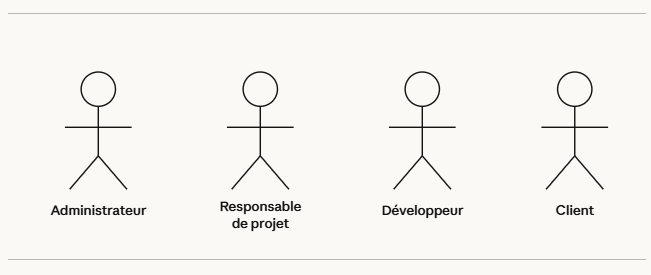
\includegraphics[width=0.9\textwidth,keepaspectratio]{Images/acteurs.png}
\caption{Illustration des acteurs du système SolidMaint}
\label{fig:acteurs}
\end{figure}

\subsection{Identification des besoins fonctionnels}
L'identification des besoins fonctionnels constitue une étape fondamentale dans la
conception de \textbf{SolidMaint}. Ces spécifications définissent précisément les
opérations que la plateforme doit être capable d'exécuter pour répondre aux exigences
métier de SolidWall Consulting.

\subsubsection{Authentification et Gestion de Compte}

Ce module assure l'authentification sécurisée via identifiants classiques ou OAuth 2.0 (Google, GitHub) avec gestion automatique des jetons d'accès. Lors de la première connexion, le système impose un changement de mot de passe pour les comptes créés par un administrateur. Un processus de réinitialisation obligatoire bloque l'accès à l'application jusqu'à la définition d'un mot de passe personnel, garantissant que seul l'utilisateur légitime détient les informations d'authentification définitives.

\begin{figure}[H]
    \centering
    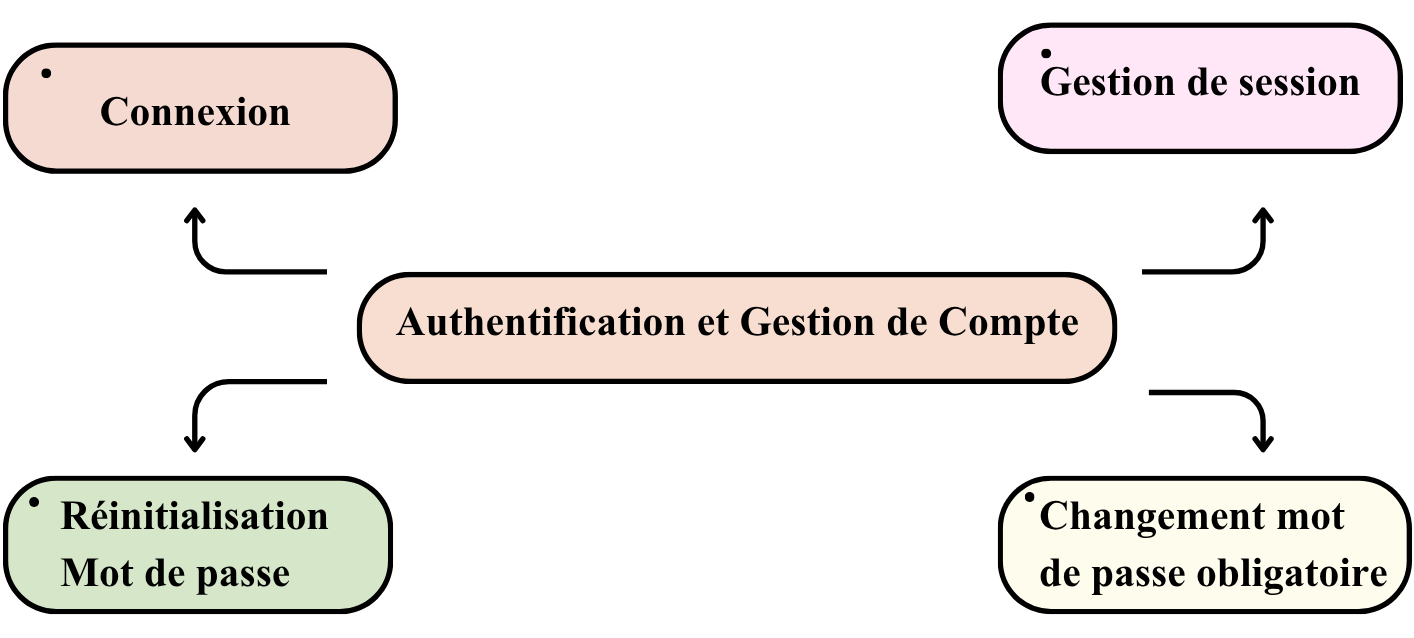
\includegraphics[width=0.7\textwidth,keepaspectratio]{Images/soumission_demande_inscription.png}
    \caption{Authentification et Gestion de Compte}
    \label{fig:authentification_gestion_compte}
\end{figure}

\vspace{0.5cm}

\subsubsection{Gestion des Utilisateurs et Demandes d'Inscription}

Ce module permet aux administrateurs de gérer le cycle de vie complet des comptes utilisateurs avec création automatisée, gestion des profils et contrôle des activations/désactivations. Le traitement des demandes d'inscription s'effectue via une interface centralisée permettant approbation, rejet ou mise en attente avec notifications automatiques.

\begin{figure}[H]
    \centering
    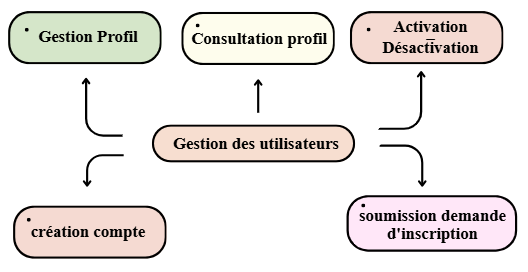
\includegraphics[width=0.7\textwidth,keepaspectratio]{Images/inscription_creation_utilisateur.png}
    \caption{Gestion des Utilisateurs et Demandes d'Inscription}
    \label{fig:gestion_utilisateurs}
\end{figure}

\vspace{0.5cm}

\subsubsection{Système de Rôles et Permissions}

Les droits sont gérés par rôles selon un modèle RBAC (Role-Based Access Control) : chaque rôle regroupe un ensemble de permissions, ce qui permet d’attribuer finement les accès. La conception modulaire permet aux administrateurs de créer des rôles personnalisés en combinant dynamiquement les permissions existantes selon les besoins organisationnels spécifiques. Cette flexibilité permet d'ajuster les autorisations d'un rôle sans impact sur les autres configurations, facilitant l'évolution du système de sécurité.

\begin{figure}[H]
    \centering
    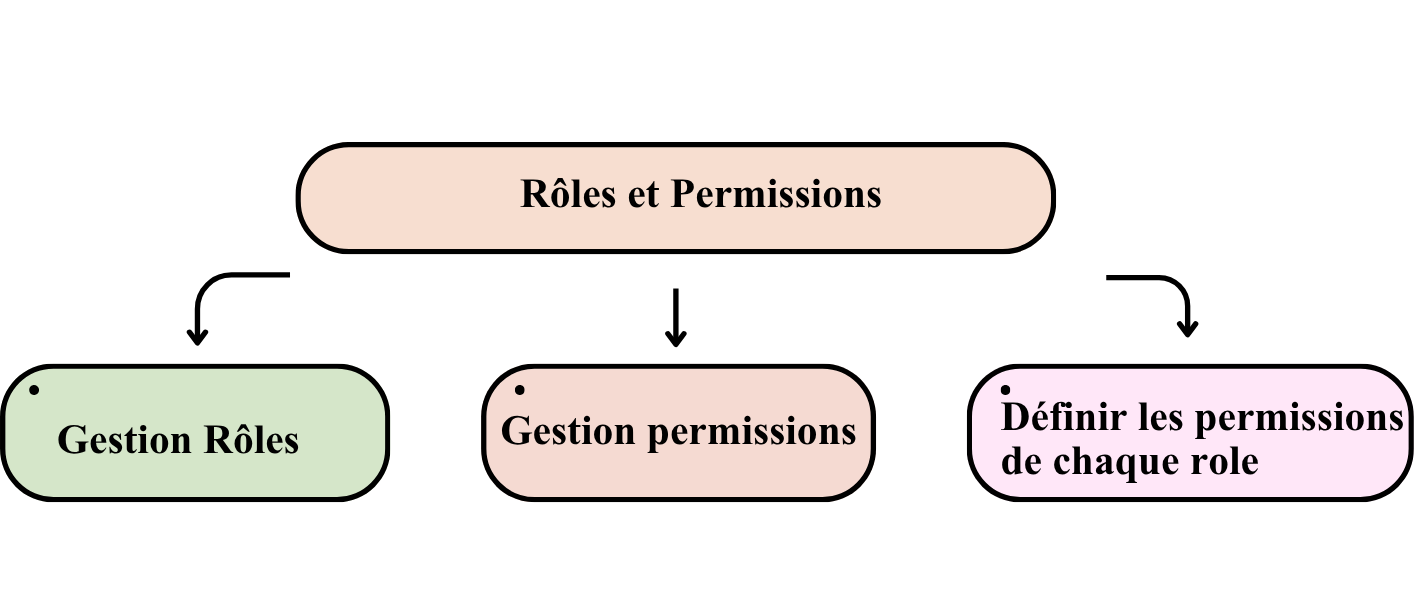
\includegraphics[width=0.7\textwidth,keepaspectratio]{Images/gestion_permissions.png}
    \caption{Système de Rôles et Permissions}
    \label{fig:roles_permissions}
\end{figure}

\vspace{0.5cm} 

\subsubsection{Gestion des Clients et Projets}

Ce module centralise la gestion des clients avec création automatisée des comptes. Le système génère des organigrammes visuels et interactifs pour chaque projet, présentant la hiérarchie complète (client, chef de projet, équipe) avec accès direct aux coordonnées de tous les interlocuteurs. Cette visualisation facilite l'identification rapide des contacts et optimise la communication en cas de problème.

\begin{figure}[H]
    \centering
    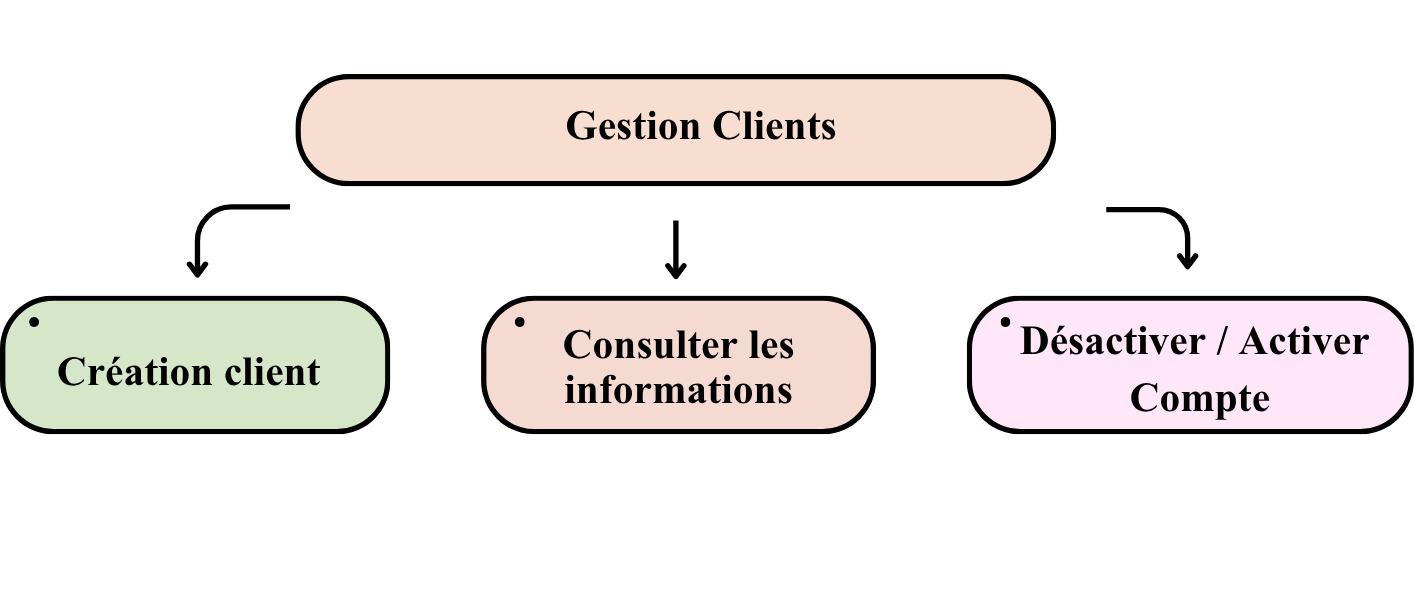
\includegraphics[width=0.7\textwidth,keepaspectratio]{Images/gestion_client.png}
    \caption{Gestion des Clients et Projets}
    \label{fig:gestion_clients}
\end{figure}

\subsubsection{Gestion des Contrats de Maintenance}

Ce module automatise le cycle de vie complet des contrats de maintenance avec système d'alertes préventives échelonnées. L'import de contrats s'effectue à partir de fichiers PDF, avec extraction automatique de données pour pré-remplir les formulaires de création.
\begin{figure}[H]
    \centering
    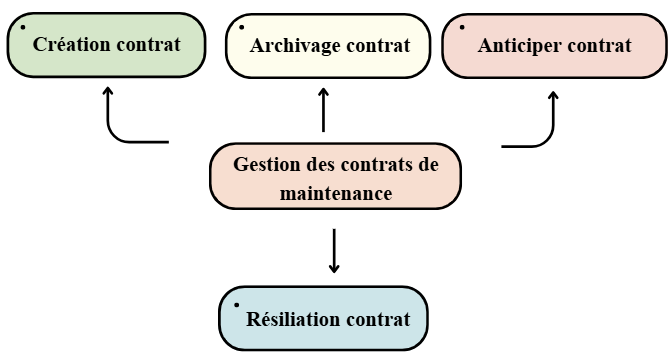
\includegraphics[width=0.7\textwidth,keepaspectratio]{Images/gestion_contrat.png}
    \caption{Gestion des contrats de maintenance}
    \label{fig:gestion_contrats}
\end{figure}

\subsubsection{Gestion des Demandes d'Intervention}

Ce module structure la soumission des demandes d'intervention avec vérification automatique de couverture contractuelle et validation des types d'intervention éligibles. Le processus de validation intègre un système de relance automatique garantissant le traitement dans les délais impartis avec escalade vers les responsables en cas de dépassement des seuils temporels.

\begin{figure}[H]
    \centering
    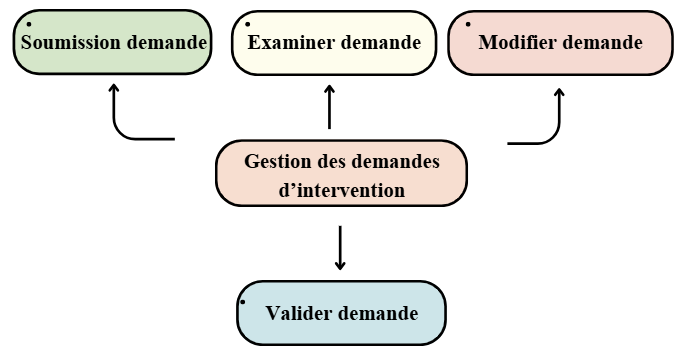
\includegraphics[width=0.7\textwidth,keepaspectratio]{Images/gestion_demande.png}
    \caption{Gestion des demandes d'intervention}
    \label{fig:gestion_demandes}
\end{figure}

\subsubsection{Gestion Avancée des Tickets de Maintenance}

Ce module recommande automatiquement les développeurs les plus adaptés à un ticket, permet de suivre le temps de travail via chronométrage, et de signaler des blocages avec analyse automatique par IA. Les solutions sont proposées collaborativement entre membres de l'équipe. La soumission en revue déclenche la clôture automatique des sessions et le calcul du temps cumulé. Après validation par le chef de projet, le client peut fermer le ticket, signaler un problème persistant, ou obtenir une extension automatique de sept jours.
\subsubsection{Tableaux de Bord, Traçabilité et Documentation}

Ce module offre des tableaux de bord personnalisés par rôle avec indicateurs clés de performance. Il maintient un historique exhaustif de toutes les opérations avec traçabilité complète et système de notifications multicanaux (web, email, Slack). La génération automatique de procès-verbaux PDF s'effectue à partir des informations de tickets lors de la résolution, produisant une documentation contractuelle structurée.

\begin{figure}[H]
    \centering
    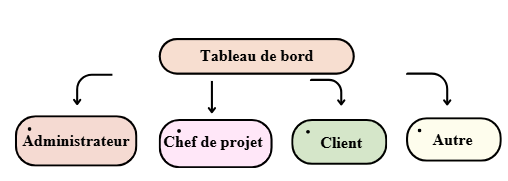
\includegraphics[width=0.7\textwidth,keepaspectratio]{Images/dashboard.png}
    \caption{Tableau de bord et reportage}
    \label{fig:dashboard}
\end{figure}

\begin{figure}[H]
    \centering
    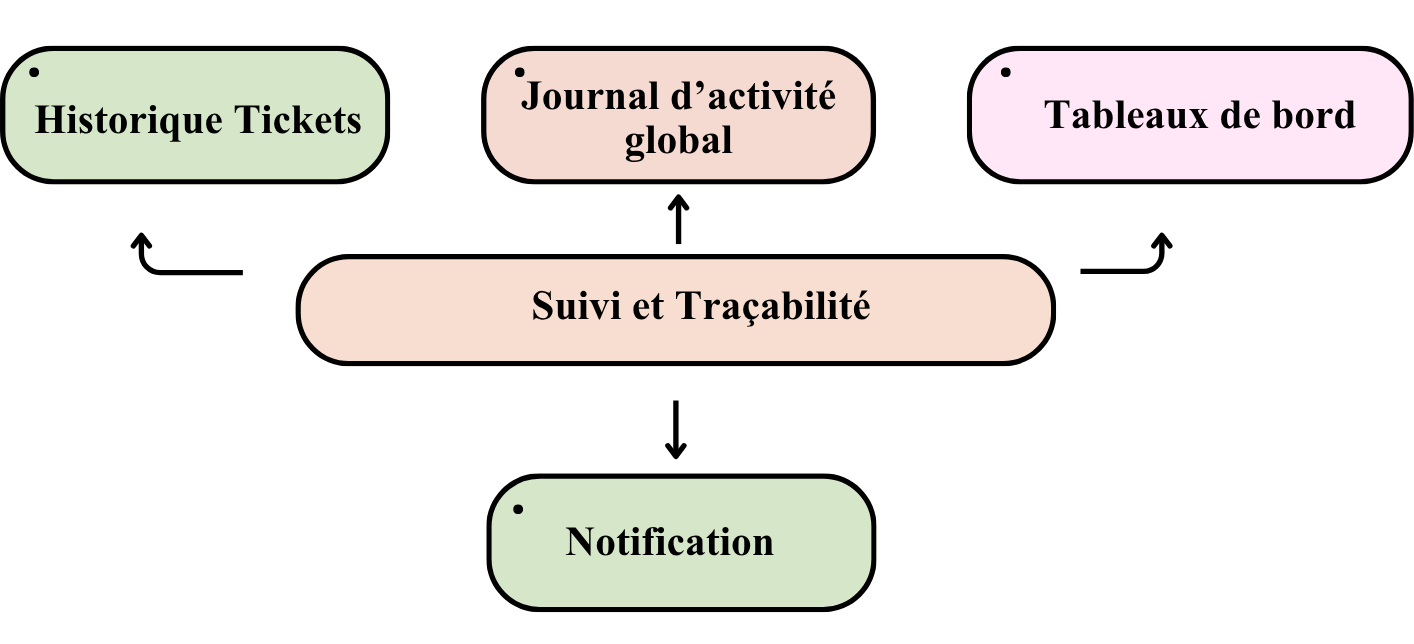
\includegraphics[width=0.7\textwidth,keepaspectratio]{Images/suivi_tracabilite.png}
    \caption{Suivi et Traçabilité}
    \label{fig:suivi_tracabilite}
\end{figure}

\begin{figure}[H]
    \centering
    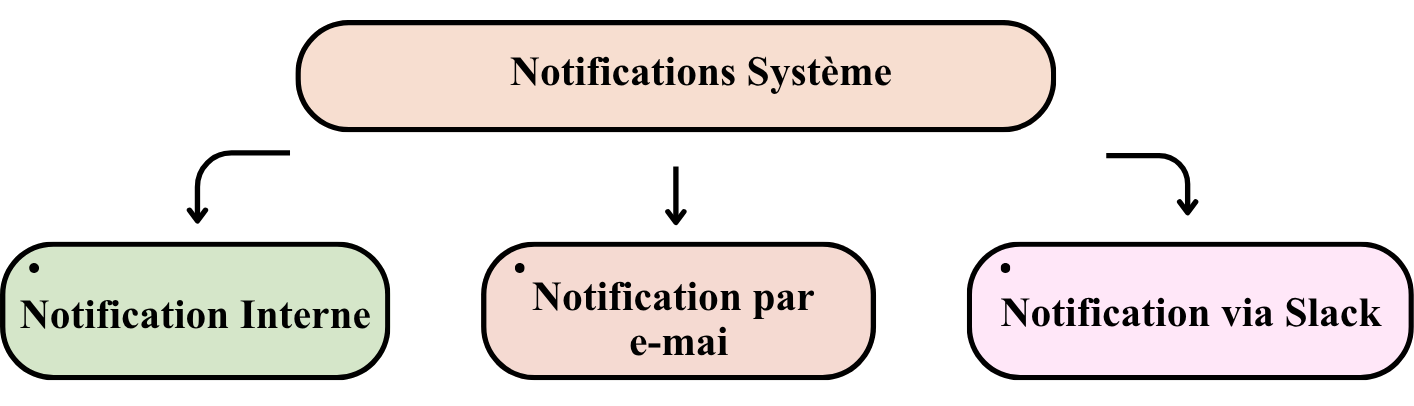
\includegraphics[width=0.7\textwidth,keepaspectratio]{Images/notifications.png}
    \caption{Notifications Système}
    \label{fig:notifications}
\end{figure}

\subsection{Identification des besoins non fonctionnels}
Afin de garantir la qualité logicielle, la robustesse et la pérennité de la plateforme, plusieurs exigences non fonctionnelles ont été définies et prises en compte lors de la conception et du développement :

\begin{itemize}[label=$\blacktriangleright$]

\item \textbf{Ergonomie et Accessibilité :} 
L'interface utilisateur doit offrir une utilisabilité optimale, caractérisée par une navigation fluide, une cohérence visuelle et une architecture adaptative (\textit{responsive design}). La plateforme doit intégrer des mécanismes de confort visuel, notamment à travers un système de thématisation dynamique (modes clair et sombre), et supporter nativement l'internationalisation pour garantir une accessibilité multilingue.

\item \textbf{Sécurité :} 
Le système doit assurer une protection rigoureuse de l'application et des données à travers des mécanismes d'authentification forte, une gestion stricte des autorisations basée sur les rôles (RBAC), et le chiffrement des informations sensibles. La traçabilité des actions critiques doit être garantie par un système de journalisation (\textit{logging}) permanent afin de permettre l'audit des événements et de détecter toute anomalie ou tentative d'accès non autorisé.

\item \textbf{Performance et Évolutivité :} 
Afin de garantir des latences minimales, même sous affluence critique, l'architecture doit intégrer des stratégies d'optimisation de l'accès aux données (mise en cache, requêtes optimisées) prenant en compte la sollicitation liée à l'opération d'indexation, tout en supportant une montée en charge progressive.

\item \textbf{Réactivité et Temps Réel :} 
Pour les modules nécessitant une synchronisation instantanée (tels que les notifications ou les alertes de gestion), le système doit garantir une communication bidirectionnelle à faible latence entre le serveur et les clients afin d'assurer la transmission immédiate des flux d'informations.

\item \textbf{Maintenabilité et Extensibilité :} 
Le code source doit être structuré de manière modulaire en respectant les standards de conception logicielle (notamment les principes SOLID). Cela assure une maintenance facilitée, une documentation claire des interfaces (API) et une couverture de tests automatisés pour prévenir les régressions lors des évolutions futures.

\end{itemize}

%─────────────────────────────────────────────────────────────────────────────
% SECTION II : MODÉLISATION DES BESOINS
%─────────────────────────────────────────────────────────────────────────────

\section{Modélisation des besoins}
\label{sec:modelisation_besoins}
L'analyse des besoins fonctionnels se poursuit par une modélisation dynamique à
l'aide du diagramme de cas d'utilisation UML. Ce diagramme offre une vision
synthétique des fonctionnalités offertes par le système du point de vue de chaque
acteur, sans se préoccuper de leur ordre d'exécution ou des détails techniques.

La figure \ref{fig:use_case} présente le diagramme de cas d'utilisation global de
notre plateforme de service desk. Ce diagramme structure les interactions entre les
six acteurs identifiés et le système. Chaque acteur possède un périmètre d'actions
bien défini.

\begin{figure}[H]
\centering
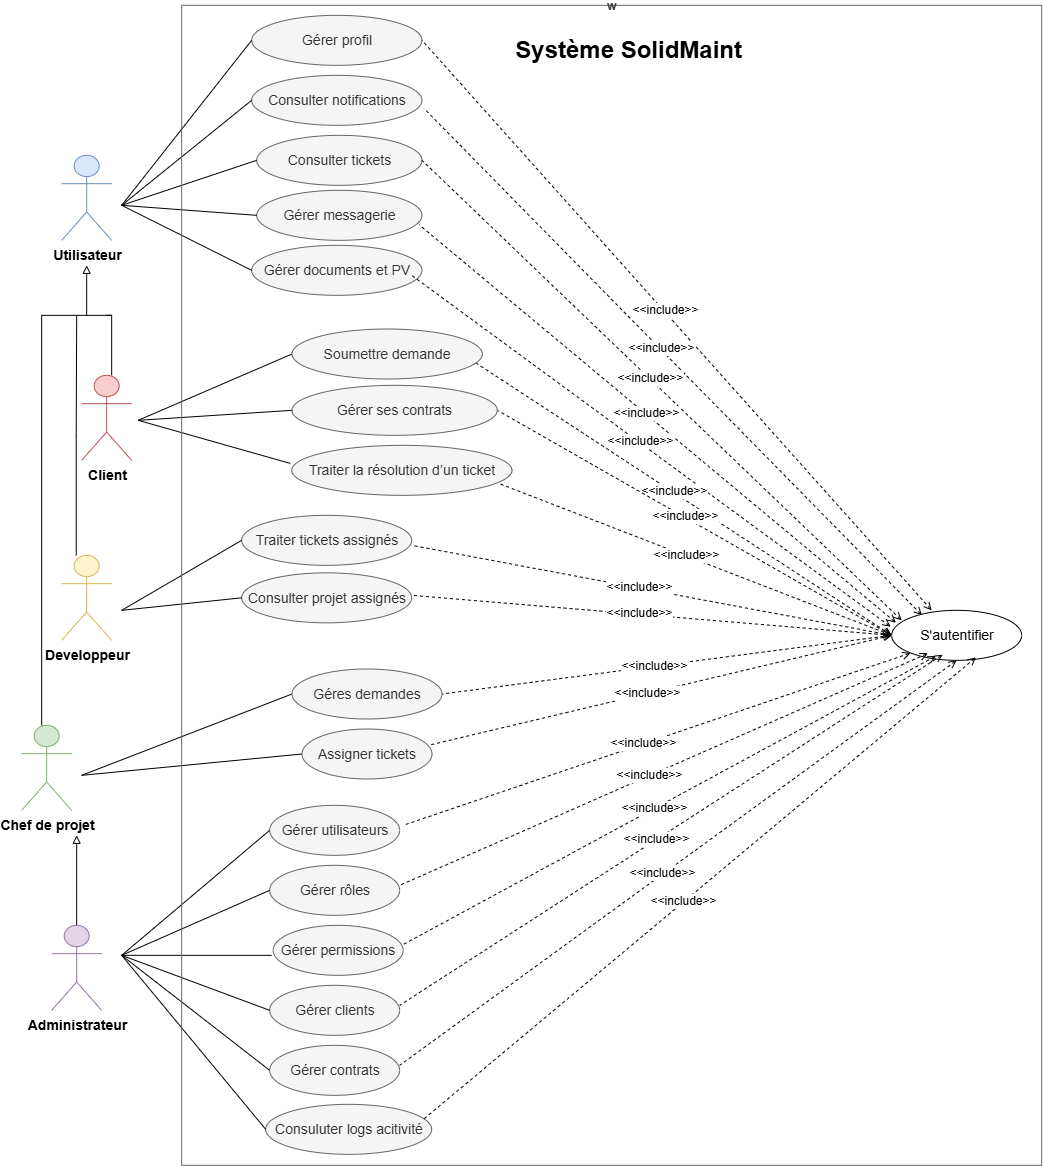
\includegraphics[width=1.0\textwidth,height=0.85\textheight,keepaspectratio]
  {Images/diagramme_cas_utilisation.png}
\caption{Diagramme de cas d'utilisation global du système}
\label{fig:use_case}
\end{figure}

%─────────────────────────────────────────────────────────────────────────────
% SECTION III : PILOTAGE AVEC SCRUM
%─────────────────────────────────────────────────────────────────────────────

\section{Pilotage du projet avec Scrum}
\label{sec:pilotage_scrum}

\subsection{Rôles de SCRUM}
Dans notre projet, Monsieur Mejdi Dhokar sera le Product Owner, Madame Maissa Ben
Fredj sera le Scrum Master, et nous, Rihab Chourou et Eya Gharbi, formons l'équipe
de développement.

\begin{figure}[H]
\centering
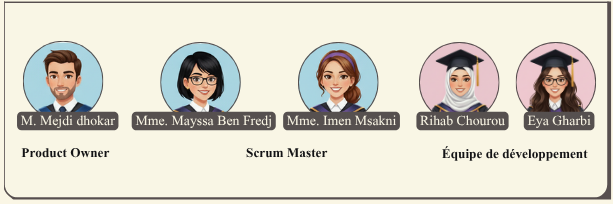
\includegraphics[width=0.9\textwidth,keepaspectratio]{Images/Equipe_Scrum.png}
\caption{Équipe Scrum et rôles}
\end{figure}

\subsubsection{Backlog de produit}
Comme évoqué dans le premier chapitre, le Product Backlog constitue l'un des
artefacts fondamentaux de la méthodologie Scrum. Il permet de formaliser les
exigences fonctionnelles ainsi que les fonctionnalités attendues du système. Le
tableau ci-dessous présente le Product Backlog de notre solution \textbf{SolidMaint},
structuré selon les éléments suivants :

\begin{itemize}[nosep,leftmargin=1.6cm,topsep=0pt,itemsep=2pt,label=$\bullet$]
  \item \textbf{Id EPIC} : Identifiant unique attribué à chaque EPIC afin de
    faciliter son identification et sa gestion dans le système de projet.
  \item \textbf{EPIC} : Ensemble de tâches interconnectées visant à atteindre un
    objectif majeur dans la gestion agile de projet ou le développement logiciel.
  \item \textbf{Id User Story} : Valeur unique et incrémentale associée à chaque
    user story pour assurer sa traçabilité.
  \item \textbf{User Story} : Description de la fonctionnalité du point de vue de
    l'utilisateur final, suivant le format ``En tant que [rôle], je souhaite [action]
    afin de [bénéfice]''.
  \item \textbf{Critères d'acceptation} : Conditions spécifiques et mesurables qui
    doivent être remplies pour que la user story soit considérée comme terminée et
    acceptée par le Product Owner.
  \item \textbf{Priorité} : Niveau d'importance défini par le Product Owner pour
    chaque tâche, permettant de prioriser les développements.
\end{itemize}

\noindent\textbf{Légende des priorités :} + : Faible \quad ++ : Moyenne \quad
+++ : Élevée.

\rowcolors{0}{}{}
\arrayrulecolor{black}
\renewcommand{\arraystretch}{1.2}
\small

% Au début de la longtable, remplace l'en-tête par :
\begin{longtable}{|C{1cm}|C{2.8cm}|M{1.2cm}|>{\raggedright\arraybackslash}p{4.7cm}|>{\raggedright\arraybackslash}p{4.5cm}|M{1.3cm}|}

   
    \rowcolor{lightblue}
    \textbf{ID Epic} & \textbf{Épic} & \textbf{ID US} & \multicolumn{1}{c|}{\textbf{User Story}} & \multicolumn{1}{c|}{\textbf{Critères d'acceptation}} & \textbf{Priorité} \\
    \hline
    \endfirsthead

    \hline
    \endhead

\hline
\endfoot

\hline
\endlastfoot

% Epic 1: Authentification et Sécurité
\multirow{5}{*}{\centering 1} & \multirow{5}{2.5cm}{\centering Authentification et Sécurité} 
& US01 & En tant qu'\textbf{utilisateur}, je souhaite m'authentifier avec email et mot de passe afin d'accéder à mes informations de manière sécurisée. 
& L'utilisateur authentifié avec succès accède à son tableau de bord personnalisé selon son rôle. & +++ \\
\cline{3-6}
& & US02 & En tant qu'\textbf{utilisateur}, je souhaite réinitialiser mon mot de passe afin de retrouver l'accès à mon compte. 
& L'utilisateur reçoit un email avec un lien valide 24h et peut définir un nouveau mot de passe conforme aux règles de sécurité. & +++ \\
\cline{3-6}
& & US03 & En tant qu'\textbf{utilisateur}, je souhaite m'authentifier via Google ou GitHub afin de me connecter rapidement sans créer de compte. 
& L'utilisateur peut se connecter via son compte Google ou GitHub et accéder immédiatement à l'application. & ++ \\
\cline{3-6}
& & US04 & En tant qu'\textbf{utilisateur}, je souhaite me déconnecter de la plateforme afin de sécuriser ma session. 
& Après déconnexion, l'utilisateur ne peut plus accéder aux pages protégées sans se reconnecter. & ++ \\
\cline{3-6}
& & US05 & En tant qu'\textbf{utilisateur}, je souhaite que mon compte soit protégé contre les tentatives de connexion malveillantes afin de garantir la sécurité de mes données. 
& Après 3 tentatives échouées, le compte est temporairement verrouillé et l'utilisateur reçoit une notification par email. & +++ \\
\hline

\multirow{2}{*}{\centering 2} & \multirow{5}{2.5cm}{\centering Gestion des utilisateurs } 

% Epic 2: Gestion des utilisateurs 

& US06 & En tant qu'\textbf{utilisateur}, je souhaite gérer mon profil afin que mes informations soient toujours à jour. 
& L'utilisateur peut modifier et sauvegarder ses informations personnelles qui sont validées avant enregistrement. & ++ \\
\cline{3-6}
& & US07 & En tant qu'\textbf{utilisateur}, je souhaite consulter l'historique de mes activités afin de suivre mes actions dans le système. 
& L'utilisateur visualise toutes ses actions passées avec possibilité de filtrer par date et type d'action. & ++ \\

\cline{3-6}
& & US08 & En tant qu'\textbf{administrateur}, je souhaite créer des utilisateurs afin de gérer les accès au système. 
& Le nouvel utilisateur reçoit un email d'invitation avec un mot de passe temporaire pour sa première connexion. & +++ \\
\cline{3-6}
& & US09 & En tant qu'\textbf{administrateur}, je souhaite modifier les informations d'un utilisateur afin de maintenir des données à jour. 
& Les modifications sont enregistrées avec traçabilité et l'utilisateur concerné est notifié des changements. & ++ \\
\cline{3-6}
& & US10 & En tant qu'\textbf{administrateur}, je souhaite activer et désactiver un compte utilisateur afin de contrôler l'accès au système. 
& Un compte désactivé ne peut plus se connecter et l'utilisateur reçoit une notification du changement de statut. & +++ \\
\cline{3-6}
& & US11 & En tant qu'\textbf{administrateur}, je souhaite consulter la liste des utilisateurs afin de visualiser et gérer efficacement les comptes. 
& La liste complète des utilisateurs est affichée avec possibilité de filtrer, rechercher et exporter les données. & ++ \\
\hline

% Epic 3: Gestion des rôles et permissions 
\multirow{5}{*}{\centering 3} & \multirow{5}{2.5cm}{\centering Gestion des rôles et permissions} 
& US12 & En tant qu'\textbf{administrateur}, je souhaite gérer des rôles afin de structurer les accès au système. 
& L'administrateur peut créer, modifier et archiver des rôles avec vérification des utilisateurs associés. & +++ \\
\cline{3-6}
& & US13 & En tant qu'\textbf{administrateur}, je souhaite attribuer des permissions granulaires aux rôles afin de contrôler précisément les accès. 
& L'administrateur sélectionne les permissions par catégorie et visualise un aperçu avant validation. & +++ \\
\cline{3-6}
& & US14 & En tant qu'\textbf{administrateur}, je souhaite consulter la matrice rôles-permissions afin de visualiser rapidement les droits de chaque rôle. 
& La matrice affiche clairement tous les rôles et leurs permissions avec possibilité de filtrer et exporter. & ++ \\
\hline
\enlargethispage{2cm}
% Epic 4: Demandes d'inscription OAuth
\multirow{2}{*}{\centering 4} & \multirow{2}{2.5cm}{\centering Gestion des demandes d'inscription OAuth} 
& US15 & En tant qu'\textbf{utilisateur externe}, je souhaite demander l'accès via OAuth afin de m'inscrire facilement. 
& La demande est enregistrée et l'administrateur reçoit une notification pour traitement. & ++ \\
\cline{3-6}
& & US16 & En tant qu'\textbf{administrateur}, je souhaite valider ou rejeter les demandes d'inscription OAuth afin de contrôler les accès. 
& L'utilisateur reçoit un email de confirmation ou rejet et peut accéder à l'application si validé. & +++ \\
\hline

% Epic 5: Gestion des clients et projets
\multirow{7}{*}{\centering 5} & \multirow{7}{2.5cm}{\centering Gestion des Clients et projets} 
& US17 & En tant qu'\textbf{administrateur}, je souhaite créer un profil client afin de centraliser ses informations. 
& Le profil client est créé avec toutes les informations nécessaires et un identifiant unique est généré. & +++ \\
\cline{3-6}
& & US18 & En tant qu’administrateur, je souhaite consulter la liste des clients  afin de visualiser les clients existants. 
& La liste complète des clients est accessible avec possibilité de filtrer, rechercher et exporter. & ++ \\
\cline{3-6}
& & US19 & En tant qu'\textbf{administrateur}, je souhaite consulter le profil détaillé d'un client afin de visualiser toutes ses informations. 
& Toutes les informations du client sont affichées incluant contrats, projets et historique des interactions. & ++ \\
\cline{3-6}
& & US20 & En tant qu'\textbf{administrateur}, je souhaite modifier les informations d'un client afin de maintenir des données à jour. 
& Les modifications sont enregistrées avec traçabilité et le client est notifié si ses coordonnées changent. & ++ \\
\cline{3-6}
& & US21 & En tant qu'\textbf{administrateur}, je souhaite activer et désactiver un compte client afin de contrôler l'accès. 
& Un compte client désactivé ne peut plus accéder au système et reçoit une notification du changement. & +++ \\
\cline{3-6}
& & US22 & En tant qu'\textbf{administrateur}, je souhaite imprimer l'annuaire d'un client afin de disposer d'une version papier. 
& Un document PDF professionnel contenant toutes les informations du client est généré. & + \\

\cline{3-6}
& &US23 & En tant qu'\textbf{administrateur}, je souhaite créer un projet rattaché à un client afin d'organiser les interventions. 
& Le projet est créé et rattaché au client avec un chef de projet assigné. & +++ \\
\cline{3-6}
& & US24 & En tant qu'\textbf{administrateur}, je souhaite consulter la liste des projets afin de piloter l'activité. 
& La liste complète des projets est affichée avec possibilité de filtrer par client, statut ou chef de projet. & ++ \\
\cline{3-6}
& & US25 & En tant qu'\textbf{administrateur}, je souhaite affecter des développeurs à un projet afin de constituer l'équipe. 
& Les développeurs sont affectés au projet et peuvent visualiser les informations du projet. & +++ \\
\cline{3-6}
& & US26 & En tant que \textbf{Développeur}, je souhaite consulter les informations du projet afin de comprendre le contexte. 
& Toutes les informations du projet sont accessibles incluant client, objectifs, équipe et contrat. & ++ \\
\hline
% Epic 6: Gestion des contrats
\multirow{7}{*}{\centering 6} & \multirow{7}{2.5cm}{\centering Gestion des Contrats} 

 & US27 & En tant qu'\textbf{administrateur}, je souhaite créer un contrat de maintenance afin de formaliser les engagements de service avec le client. 
& Le contrat est créé avec client, dates, type SLA, cycle facturation et configuration des alertes d'expiration. & +++ \\
\cline{3-6}
& & US28 & En tant qu'\textbf{administrateur}, je souhaite consulter la liste des contrats afin de suivre les engagements contractuels.
& La liste affiche tous les contrats avec filtres, indicateurs visuels d'expiration et possibilité d'export. & ++ \\
\cline{3-6}
& & US29 & En tant qu'\textbf{administrateur}, je souhaite recevoir des alertes avant l'expiration des contrats afin d'anticiper les renouvellements. 
& Des alertes automatiques sont envoyées à J-30, J-15 et J-7 par email, in-app et Slack. & +++ \\
\cline{3-6}
& & US30 & En tant qu'\textbf{administrateur}, je souhaite archiver un contrat afin de conserver l'historique. 
& Le contrat est archivé avec un changement de statut, avec possibilité de restauration ultérieure. & ++ \\
\cline{3-6}
& & US31 & En tant que \textbf{client}, je souhaite demander la résiliation de mon contrat afin d'interrompre le service. 
& La demande de résiliation est créée avec motif et date souhaitée, l'administrateur reçoit une notification et peut traiter la demande. & +++ \\
\cline{3-6}
& & US32 & En tant qu'\textbf{administrateur}, je souhaite résilier un contrat afin de l'interrompre avant terme. 
& Le contrat est résilié avec date et motif, les tickets ouverts sont clôturés et le client est notifié. & +++ \\
\cline{3-6}
& & US33 & En tant que \textbf{chef de projet}, je souhaite consulter les contrats dans un calendrier afin de visualiser les dates d'expiration.
& Le calendrier affiche les contrats avec leur date d'expiration. Les contrats proches de l'expiration sont mis en évidence. L'administrateur peut exporter le calendrier. & ++ \\
\cline{3-6}
& & US34 & En tant que \textbf{client}, je souhaite soumettre un retour d'expérience à l'expiration de mon contrat afin d'exprimer ma satisfaction.
& Le retour d’expérience est accessible pour les contrats expirés ou proches de l’expiration. Un seul retour d’expérience par contrat est accepté. & ++\\
\cline{3-6}
& & US35 & En tant qu'\textbf{administrateur}, je souhaite générer un PDF formaté du contrat afin de le partager avec le client.
& Le PDF généré contient les informations necessaires; les dates d'intervention& +\\
\cline{3-6}
& & US36 & En tant qu'\textbf{administrateur}, je souhaite consulter les détails d'un contrat afin de visualiser toutes ses informations.
& Toutes les informations du contrat sont affichées incluant client, dates, SLA, documents et historique. & ++ \\
\cline{3-6}
& & US37 & En tant qu'\textbf{équipe produit}, je souhaite réserver cet identifiant afin de conserver une numérotation continue du backlog.
& Identifiant réservé pour maintien de la cohérence de numérotation. & + \\
\hline

\multirow{8}{*}{\centering 8} & \multirow{8}{2.5cm}{\centering Gestion des demandes clients} 

% Epic 8: Gestion des demandes clients

& US38 & En tant que \textbf{client}, je souhaite soumettre une demande de maintenance afin de signaler un besoin. 
& Le client peut joindre des fichiers à sa demande. Le système génère un numéro unique de suivi. Le client reçoit une confirmation de réception. & +++ \\
\cline{3-6}
& & US39 & En tant que \textbf{chef de projet}, je souhaite consulter les demandes en attente afin de les traiter. 
& Le chef de projet visualise toutes les demandes nécessitant un traitement. Les demandes sont triées par date de création. Les demandes urgentes sont identifiables visuellement. & +++ \\
\cline{3-6}
& & US40 & En tant que \textbf{chef de projet}, je souhaite valider une demande afin de la convertir en ticket. 
& Le chef de projet peut approuver une demande. Le chef de projet définit la catégorie et la priorité. Un ticket est automatiquement créé et lié à la demande. & +++ \\
\cline{3-6}
& & US41 & En tant que \textbf{chef de projet}, je souhaite demander des informations complémentaires afin de clarifier une demande. 
& Le chef de projet peut solliciter des précisions au client. Le client est notifié de la demande d'informations. Un rappel est envoyé si aucune réponse après 48h. & ++ \\
\cline{3-6}
& & US42 & En tant que \textbf{client}, je souhaite compléter ma demande afin de fournir les informations manquantes. 
& Le client peut répondre aux questions posées. Le chef de projet est notifié de la réponse. La demande redevient disponible pour traitement. & ++ \\
\cline{3-6}
& & US43 & En tant que \textbf{chef de projet}, je souhaite requalifier une demande afin de corriger sa catégorie ou sa priorité. 
& Le chef de projet peut modifier la catégorie d'une demande. Le chef de projet peut ajuster la priorité. Une justification est obligatoire pour toute modification. Toutes les modifications sont tracées. & ++ \\
\cline{3-6}
& & US44 & En tant qu'\textbf{utilisateur}, je souhaite commenter une demande afin de communiquer sur le contexte. 
& L'utilisateur peut ajouter des commentaires à une demande. L'utilisateur peut joindre des fichiers aux commentaires. Les autres parties prenantes sont notifiées des nouveaux commentaires. & ++ \\
\cline{3-6}
& & US45 & En tant qu'\textbf{utilisateur}, je souhaite consulter l'historique d'une demande afin de suivre son évolution. 
& L'utilisateur visualise tous les événements liés à la demande. L'historique affiche la date et l'auteur de chaque action. L'utilisateur peut filtrer l'historique par type d'événement. & ++ \\
\hline
\multirow{20}{*}{\centering 9} & \multirow{20}{2.5cm}{\centering Gestion des tickets} 

% Epic 9: Gestion des tickets
 
& US46 & En tant que \textbf{développeur}, je souhaite visualiser mes tickets dans un tableau Kanban afin de gérer mes tâches. 
& Le développeur visualise ses tickets organisés par état d'avancement. Le développeur peut déplacer un ticket d'un état à un autre. Le développeur voit si un ticket risque de dépasser son délai. & +++ \\
\cline{3-6}
& & US47 & En tant que \textbf{chef de projet}, je souhaite assigner un ticket à un développeur afin de répartir la charge. 
& Le chef de projet sélectionne un développeur disponible. Le système alerte si le développeur a déjà trop de tickets. Le développeur assigné est notifié immédiatement. & +++ \\
\cline{3-6}
& & US48 & En tant que \textbf{chef de projet}, je souhaite assigner un ticket à plusieurs développeurs afin de collaborer sur des tâches complexes. 
& Le chef de projet peut assigner plusieurs développeurs au même ticket. Le chef de projet définit le rôle de chaque développeur. Le temps estimé est réparti entre les développeurs. & ++ \\
\cline{3-6}
& & US49 & En tant que \textbf{développeur}, je souhaite me désassigner d'un ticket afin de libérer ma charge. 
& Le développeur doit fournir un motif pour se désassigner. Le ticket redevient disponible pour assignation. Le chef de projet est notifié de la désassignation. & ++ \\
\cline{3-6}
& & US50 & En tant que \textbf{développeur}, je souhaite démarrer un chronomètre sur un ticket afin de tracker mon temps. 
& Le développeur peut démarrer le suivi du temps de travail. Une session de travail est créée avec l'heure de début. Le développeur voit le temps écoulé en temps réel. & +++ \\
\cline{3-6}
& & US51 & En tant que \textbf{développeur}, je souhaite mettre en pause mon chronomètre afin de gérer les interruptions. 
& Le développeur peut suspendre temporairement le suivi du temps. Le temps écoulé est enregistré. Le développeur peut reprendre le suivi ultérieurement. & ++ \\
\cline{3-6}
& & US52 & En tant que \textbf{développeur}, je souhaite arrêter le chronomètre afin de finaliser ma session. 
& Le développeur peut arrêter le suivi du temps. Le développeur peut ajouter un commentaire sur le travail effectué. La session est ajoutée à l'historique. Le développeur est alerté si le temps dépasse l'estimation. & +++ \\
\cline{3-6}
& & US53 & En tant que \textbf{développeur}, je souhaite ajouter manuellement une session de travail afin de corriger des oublis. 
& Le développeur peut enregistrer une session de travail passée. Le développeur doit fournir la date, l'heure et la durée. Le développeur doit justifier l'ajout manuel. Le système vérifie qu'il n'y a pas de chevauchement avec d'autres sessions. & ++ \\
\cline{3-6}
& & US54 & En tant que \textbf{développeur}, je souhaite changer le statut d'un ticket afin de refléter l'avancement. 
& Le développeur peut faire progresser un ticket selon le workflow défini. Le système empêche les transitions invalides. Toutes les parties prenantes sont notifiées lors d'un changement. L'historique des changements est conservé. & +++ \\
\cline{3-6}
& & US55 & En tant que \textbf{client}, je souhaite valider la résolution d'un ticket afin de confirmer que le problème est résolu. 
& Le client peut confirmer que le problème est résolu. Le client peut ajouter un commentaire de validation. Le ticket est fermé après validation. Le développeur est notifié de la validation. & +++ \\
\cline{3-6}
& & US56 & En tant que \textbf{chef de projet}, je souhaite rouvrir un ticket fermé afin de traiter un problème récurrent. 
& Le chef de projet doit justifier la réouverture. Le délai SLA est réinitialisé. Les développeurs assignés sont notifiés. & ++ \\
\cline{3-6}
& & US57 & En tant que \textbf{chef de projet}, je souhaite consulter le temps passé par ticket afin d'analyser la productivité. 
& Le chef de projet visualise le temps total passé sur chaque ticket. Le chef de projet voit le détail par développeur. Les données sont présentées sous forme de graphiques. & ++ \\
\cline{3-6}
& & US58 & En tant que \textbf{développeur}, je souhaite signaler un blocage afin d'alerter sur un obstacle. 
& Le développeur peut signaler un obstacle bloquant. Le développeur précise le type et l'impact du blocage. Le chef de projet reçoit une notification urgente. Le délai SLA est suspendu pendant le blocage. & +++ \\
\cline{3-6}
& & US59 & En tant que \textbf{membre d'équipe}, je souhaite résoudre un blocage afin de permettre au développeur de reprendre son travail. 
& Le blocage est résolu avec commentaire obligatoire, le chrono SLA reprend et l'action est tracée. & ++ \\
\cline{3-6}
& & US60 & En tant que \textbf{développeur}, je souhaite demander une extension de délai SLA afin de disposer de plus de temps. 
& La demande d'extension est créée avec durée et justification pour validation par le chef de projet. & ++ \\
\cline{3-6}
& & US61 & En tant que \textbf{chef de projet}, je souhaite approuver ou rejeter les demandes d'extension SLA. 
& La liste des demandes en attente est affichée, l'approbation ou rejet avec commentaire met à jour automatiquement le SLA. & ++ \\
\cline{3-6}
& & US62 & En tant qu'\textbf{utilisateur}, je souhaite commenter un ticket avec mentions afin de communiquer efficacement. 
& Les commentaires sont ajoutés avec éditeur riche, autocomplétion @utilisateur et distinction internes/externes. & +++ \\
\cline{3-6}
& & US63 & En tant qu'\textbf{utilisateur}, je souhaite ajouter des pièces jointes aux tickets afin de fournir du contexte. 
& Les fichiers sont ajoutés par drag \& drop (images/PDF/logs, max 10MB) avec prévisualisation. & ++ \\
\cline{3-6}
& & US64 & En tant que \textbf{développeur}, je souhaite être informé lorsqu'un autre utilisateur modifie le même ticket. 
& Une notification temps réel via WebSocket affiche un toast et un indicateur "X est en train d'éditer". & ++ \\
\cline{3-6}
& & US65 & En tant qu'\textbf{utilisateur}, je souhaite consulter l'historique complet d'un ticket afin de comprendre son évolution. 
& La timeline chronologique inversée affiche tous les événements avec filtres par type et export PDF. & ++ \\
\hline

% Epic 13: Dashboards et rapports - Calendrier et planification

\multirow{4}{*}{\centering 13} & \multirow{4}{2.5cm}{\centering Calendrier et planification}  
& US66 & En tant qu'\textbf{utilisateur}, je souhaite visualiser les tickets et demandes de maintenance sur un calendrier mensuel afin d'avoir une vue globale des interventions 
& L'utilisateur peut naviguer entre les mois, distinguer les types d'événements (Tickets/Demandes) par couleur et voir les titres tronqués. & +++ \\
\cline{3-6}
& & US67 & En tant qu'\textbf{administrateur}, je souhaite identifier visuellement les urgences SLA sur le calendrier afin de prioriser les interventions critiques. 
& Les événements en retard ou proches de l'échéance apparaissent en rouge/orange avec un indicateur visuel (pulse) sur les urgences critiques. & +++ \\
\cline{3-6}
& & US68 & En tant que \textbf{Chef de Projet}, je souhaite accéder à une vue Gantt / Agenda afin d'analyser la charge de travail et la progression de chaque développeur. 
&La vue affiche la timeline des affectations, le pourcentage de progression des tickets et le taux de charge calculé en temps réel par développeur. & ++ \\
\cline{3-6}
& & US69 & En tant qu'\textbf{utilisateur}, je souhaite accéder aux détails d'un ticket directement depuis le calendrier afin de consulter ou modifier l'intervention rapidement. 
& Un clic sur un événement dans le calendrier ou le panneau latéral redirige l'utilisateur vers la page de détails correspondante. & ++ \\
\hline
% Epic 10: Messagerie et collaboration
\multirow{9}{*}{\centering 10} & \multirow{9}{2.5cm}{\centering Messagerie et collaboration} 

& US70 & En tant qu'\textbf{utilisateur}, je souhaite accéder à une messagerie intégrée afin de communiquer avec mon équipe. 
& L'utilisateur visualise les canaux de discussion disponibles. L'utilisateur voit le nombre de messages non lus. L'utilisateur identifie les membres présents. & ++ \\
\cline{3-6}
& & US71 & En tant qu'\textbf{utilisateur}, je souhaite envoyer des messages dans un channel afin de communiquer. 
& L'utilisateur peut rédiger et envoyer des messages. L'utilisateur peut joindre des fichiers. Les messages sont reçus instantanément par les autres membres. & +++ \\
\cline{3-6}
& & US72 & En tant qu'\textbf{utilisateur}, je souhaite répondre à un message afin de créer un fil de discussion. 
& L'utilisateur peut répondre à un message spécifique. Les réponses sont regroupées dans un fil dédié. Seuls les participants au fil reçoivent les notifications. & ++ \\
\cline{3-6}
& & US73 & En tant qu'\textbf{utilisateur}, je souhaite mentionner des collègues afin d'attirer leur attention. 
& L'utilisateur peut mentionner un collègue dans un message. Le collègue mentionné reçoit une notification. Le message mentionné est mis en évidence pour le destinataire. & +++ \\
\cline{3-6}
& & US74 & En tant qu'\textbf{utilisateur}, je souhaite éditer mes messages afin de corriger des erreurs. 
& L'utilisateur peut modifier un message récemment envoyé. Le message modifié est identifiable. L'historique des modifications est conservé. & + \\
\cline{3-6}
& & US75 & En tant qu'\textbf{utilisateur}, je souhaite supprimer mes messages afin de retirer du contenu inapproprié. 
& L'utilisateur peut supprimer ses propres messages. Une confirmation est demandée avant suppression. Le message supprimé reste visible pour l'audit. & + \\
\cline{3-6}
& & US76 & En tant qu'\textbf{utilisateur}, je souhaite épingler des messages importants afin de les retrouver facilement. 
& L'utilisateur autorisé peut épingler un message. Les messages épinglés sont facilement accessibles. L'utilisateur peut retirer l'épinglage. & ++ \\
\cline{3-6}
& & US77 & En tant que \textbf{chef de projet}, je souhaite voir qui est en ligne dans mon équipe afin de savoir qui je peux solliciter. 
& Le chef de projet visualise les membres actuellement connectés. Le chef de projet peut filtrer par équipe ou projet. Le chef de projet voit l'heure de dernière activité. & ++ \\
\cline{3-6}
& & US78 & En tant qu'\textbf{utilisateur}, je souhaite voir qui est en ligne afin de savoir qui est disponible. 
& L'utilisateur voit le statut de disponibilité des autres membres. L'utilisateur peut modifier son propre statut. Le statut est visible par tous les membres. & ++ \\
\hline

\multirow{14}{*}{\centering 11} & \multirow{14}{2.5cm}{\centering Gestion des documents} 

% Epic 11: Gestion des documents
  
& US79 & En tant qu'\textbf{utilisateur}, je souhaite uploader des documents afin de centraliser les fichiers. 
& L'utilisateur peut téléverser des documents. L'utilisateur peut associer un document à un contrat, projet ou ticket. L'utilisateur peut ajouter un titre, une description et des tags. & ++ \\
\cline{3-6}
& & US80 & En tant qu'\textbf{utilisateur}, je souhaite télécharger des documents afin de les consulter hors ligne. 
& L'utilisateur peut télécharger un document individuel. L'utilisateur peut télécharger plusieurs documents simultanément. Le système vérifie les permissions avant le téléchargement. La consultation est enregistrée pour traçabilité. & ++ \\
\cline{3-6}
& & US81 & En tant qu'\textbf{utilisateur}, je souhaite gérer les versions des documents afin d'assurer la traçabilité. 
& L'utilisateur peut téléverser une nouvelle version d'un document existant. Le système numérote automatiquement les versions. L'utilisateur doit fournir un commentaire pour chaque nouvelle version. & ++ \\
\cline{3-6}
& & US82 & En tant qu'\textbf{utilisateur}, je souhaite consulter l'historique des consultations afin de voir qui a accédé au document. 
& L'utilisateur visualise qui a consulté le document. L'utilisateur voit la date et l'heure de chaque consultation. & + \\
\cline{3-6}
& & US83 & En tant qu'\textbf{utilisateur}, je souhaite archiver des documents afin de nettoyer la vue active. 
& L'utilisateur peut archiver un document. Une confirmation est demandée avant archivage. Le document archivé peut être restauré ultérieurement. & + \\
\cline{3-6}
& & US84 & En tant que \textbf{chef de projet}, je souhaite générer automatiquement un PV à partir d'un ticket afin de documenter les interventions. 
& Le chef de projet peut générer un procès-verbal depuis un ticket. Le document contient toutes les informations du ticket et les actions réalisées. Le document peut être signé électroniquement. & +++ \\
\cline{3-6}
& & US85 & En tant que \textbf{client}, je souhaite télécharger les PV de mes tickets afin de conserver une trace des interventions. 
& Le client peut accéder aux procès-verbaux depuis ses tickets. Le client visualise l'historique de tous les PV générés. Le client reçoit une notification lors de la génération d'un nouveau PV. & ++ \\
\cline{3-6}
& & US86 & En tant qu'\textbf{développeur ou chef de projet}, je souhaite consulter la base de connaissances afin de trouver des solutions existantes. 
& L'utilisateur peut rechercher par mots-clés, catégorie ou tags. Les résultats affichent titre et extrait. Un clic ouvre l'article complet. & ++ \\
\cline{3-6}
& & US87 & En tant qu'\textbf{administrateur}, je souhaite créer des articles de la base de connaissances afin d'enrichir la documentation. 
& L'administrateur peut créer des articles. La création est tracée et horodatée. L'historique des versions est conservé. & ++ \\
\cline{3-6}
& & US88 & En tant qu'\textbf{utilisateur}, je souhaite créer une nouvelle version d'un document afin de maintenir l'historique. 
& L'utilisateur peut téléverser une nouvelle version d'un document. L'utilisateur doit fournir un commentaire pour la nouvelle version. Le système numérote automatiquement les versions. Toutes les versions précédentes sont conservées. & ++ \\
\cline{3-6}
& & US89&  En tant qu'\textbf{utilisateur}, je souhaite comparer deux versions d'un document afin de voir les différences. 
& L'utilisateur peut sélectionner deux versions à comparer. Les deux versions sont affichées côte à côte. Les modifications sont mises en évidence. & + \\
\cline{3-6}
& & US90 & En tant qu'\textbf{administrateur}, je souhaite voir qui a consulté un document afin de suivre sa diffusion. 
& L'administrateur visualise la liste des consultations du document. L'historique indique la date, l'heure et l'utilisateur. Des statistiques de consultation sont disponibles. & ++ \\
\hline

% Epic 12: Notifications
\multirow{5}{*}{\centering 12} & \multirow{5}{2.5cm}{\centering Notifications et alertes} 
& US91 & En tant qu'\textbf{utilisateur}, je souhaite recevoir des notifications in-app afin d'être informé en temps réel. 
& L'utilisateur visualise le nombre de notifications non lues. L'utilisateur peut consulter la liste des notifications. L'utilisateur peut marquer une notification comme lue. L'utilisateur peut accéder directement à l'élément concerné. & +++ \\
\cline{3-6}
& & US92 & En tant qu'\textbf{utilisateur}, je souhaite recevoir des notifications par email afin d'être informé hors connexion. 
& L'utilisateur peut configurer la fréquence des notifications email. L'utilisateur reçoit des emails pour les événements importants. & ++ \\
\cline{3-6}
& & US93 & En tant que \textbf{membre technique}, je souhaite recevoir des notifications Slack afin d'être alerté sur mon outil de travail. 
& L'administrateur peut configurer l'intégration Slack par contrat ou projet. Les événements importants sont envoyés sur Slack. & ++ \\
\cline{3-6}
& & US94 & En tant qu'\textbf{utilisateur}, je souhaite recevoir des notifications push navigateur afin d'être alerté même hors onglet. 
& L'utilisateur peut autoriser les notifications navigateur. L'utilisateur reçoit des alertes pour les événements critiques. L'utilisateur peut accéder à l'application en cliquant sur la notification. & ++ \\
\cline{3-6}
& & US95 & En tant qu'\textbf{utilisateur}, je souhaite consulter l'historique de mes notifications afin de retrouver une information. 
& L'utilisateur visualise toutes ses notifications passées. L'utilisateur peut filtrer par type ou période. L'utilisateur peut rechercher dans l'historique. & ++ \\
\hline

\multirow{8}{*}{\centering 13} & \multirow{8}{2.5cm}{\centering Dashboards et rapports } 

% Epic 13: Dashboards et rapports

& US96 & En tant qu'\textbf{administrateur}, je souhaite consulter un dashboard global afin de piloter le système. 
& L'administrateur visualise les indicateurs clés du système. L'administrateur peut filtrer les données par période. L'administrateur identifie les alertes nécessitant une action. & +++ \\
\cline{3-6}
& & US97 & En tant que \textbf{chef de projet}, je souhaite consulter un dashboard d'équipe afin de piloter l'activité. 
& Le chef de projet visualise la charge de travail de son équipe. Le chef de projet suit la performance par rapport aux délais. Le chef de projet compare le temps passé au temps estimé. & +++ \\
\cline{3-6}
& & US98 & En tant que \textbf{développeur}, je souhaite consulter mon dashboard personnel afin d'organiser ma journée. 
& Le développeur visualise ses tickets assignés. Le développeur voit ses priorités du jour. Le développeur suit son temps de travail. Le développeur identifie les échéances proches. & ++ \\
\cline{3-6}
& & US99 & En tant que \textbf{client}, je souhaite consulter mon dashboard afin de suivre mes projets. 
& Le client visualise ses contrats actifs. Le client suit l'état de ses demandes et tickets. Le client accède à ses documents récents. Le client identifie ses contacts dans l'équipe. & ++ \\
\cline{3-6}
& & US100 & En tant qu'\textbf{administrateur}, je souhaite générer un rapport d'activité mensuel afin de présenter les statistiques. 
& L'administrateur génère un rapport pour une période donnée. Le rapport contient les tickets traités et le temps passé. Le rapport indique le respect des délais. Le rapport peut être exporté. & +++ \\
\cline{3-6}
& & US101 & En tant qu'\textbf{administrateur}, je souhaite générer des rapports de conformité SLA afin de justifier les performances. 
& L'administrateur génère un rapport de conformité par contrat. Le rapport affiche le taux de respect des délais. Le rapport détaille les tickets en dépassement. & +++ \\
\cline{3-6}
& & US102 & En tant que \textbf{chef de projet}, je souhaite générer des rapports d'activité afin de présenter l'avancement. 
& Le chef de projet génère un rapport pour son équipe ou projet. Le rapport affiche les tickets traités et le temps passé. Le rapport présente l'évolution de l'activité. & ++ \\
\hline

% Epic 14: Historique et audit trail
\multirow{2}{*}{\centering 14} & \multirow{2}{2.5cm}{\centering Historique et traçabilité} 
& US103 & En tant qu'\textbf{administrateur}, je souhaite consulter l'historique complet de toutes les actions afin d'assurer la traçabilité. 
& L'administrateur visualise toutes les actions effectuées dans le système. L'historique indique l'utilisateur, la date et l'action réalisée. L'historique conserve les valeurs avant et après modification. & +++ \\
\cline{3-6}
& & US104 & En tant qu'\textbf{administrateur}, je souhaite exporter les logs d'audit afin de répondre aux exigences de conformité. 
& L'administrateur peut exporter l'historique des actions. L'administrateur peut filtrer par période, utilisateur ou type d'action. Les données exportées sont sécurisées. & ++ \\
\hline

% Epic 16: Assistance intelligente
\multirow{7}{*}{\centering 16} & \multirow{7}{2.5cm}{\centering Assistance intelligente} 
& US105 & En tant que \textbf{chef de projet}, je souhaite que l'IA analyse automatiquement les blocages afin d'identifier rapidement les problèmes critiques. 
& L'analyse est automatique lors du signalement. Le résultat est affiché dans l'interface. Un résumé clair du problème est présenté. & +++ \\
\cline{3-6}
& & US106 & En tant que \textbf{chef de projet}, je souhaite que l'IA propose des actions correctives afin de débloquer rapidement un développeur. 
& L'IA affiche 1 à 3 actions suggérées par blocage. Chaque action inclut destinataire et durée estimée. Le chef de projet peut valider une action qui crée automatiquement une tâche. & +++ \\
\cline{3-6}
& & US107 & En tant que \textbf{développeur}, je souhaite qu'un brouillon de solution soit généré à la fermeture d'un ticket afin de faciliter la documentation. 
& Un brouillon est créé automatiquement contenant : problème identifié, actions réalisées, résultat. Le développeur peut modifier le brouillon avant publication. & +++ \\
\cline{3-6}
& & US108 & En tant que \textbf{chef de projet}, je souhaite que l'IA propose une classification des demandes clients afin d'accélérer leur traitement, avec validation avant transmission au client. 
& L'IA propose type/priorité/catégorie. Le chef de projet peut accepter, modifier ou rejeter. La classification validée est visible par le client. L'audit trace proposition IA vs choix final. & +++ \\
\cline{3-6}
& & US110 & En tant que \textbf{chef de projet}, je souhaite que l'IA structure automatiquement les solutions saisies en articles KB afin d'améliorer la documentation. 
& La solution brute est transformée en format structuré (Problème/Solution/Détails). Des tags sont générés automatiquement. L'auteur peut modifier avant publication. & ++ \\
\cline{3-6}
& & US111 & En tant que \textbf{chef de projet}, je souhaite que l'IA fusionne le brouillon d'un blocage avec la solution humaine afin de produire un article KB définitif. 
& La fusion est proposée pour les blocages résolus. L'article final combine l'analyse IA et la solution humaine. Le responsable peut valider ou modifier avant publication. & + \\
\hline


 \caption{Product Backlog} \label{tab:product_backlog} \\
    \hline
\end{longtable}

\subsection{Planification des sprints}
Le projet a été mené selon la méthodologie Scrum, structuré en quatre sprints successifs s'étalant sur une période globale d'environ quatres mois. Cette approche itérative suit une logique architecturale rigoureuse : la mise en place des fondations sécuritaires, le développement de la gestion contractuelle, l'implémentation du cœur métier, et enfin l'intégration des modules collaboratifs et analytiques.

Chaque itération respecte le cycle Scrum, initié par une phase de planification (\textit{Sprint Planning}) et clôturé par les phases de revue (\textit{Sprint Review}) et de rétrospective (\textit{Sprint Retrospective}).

La figure suivante présente le déroulement chronologique de nos sprints.

\begin{figure}[H]
\centering
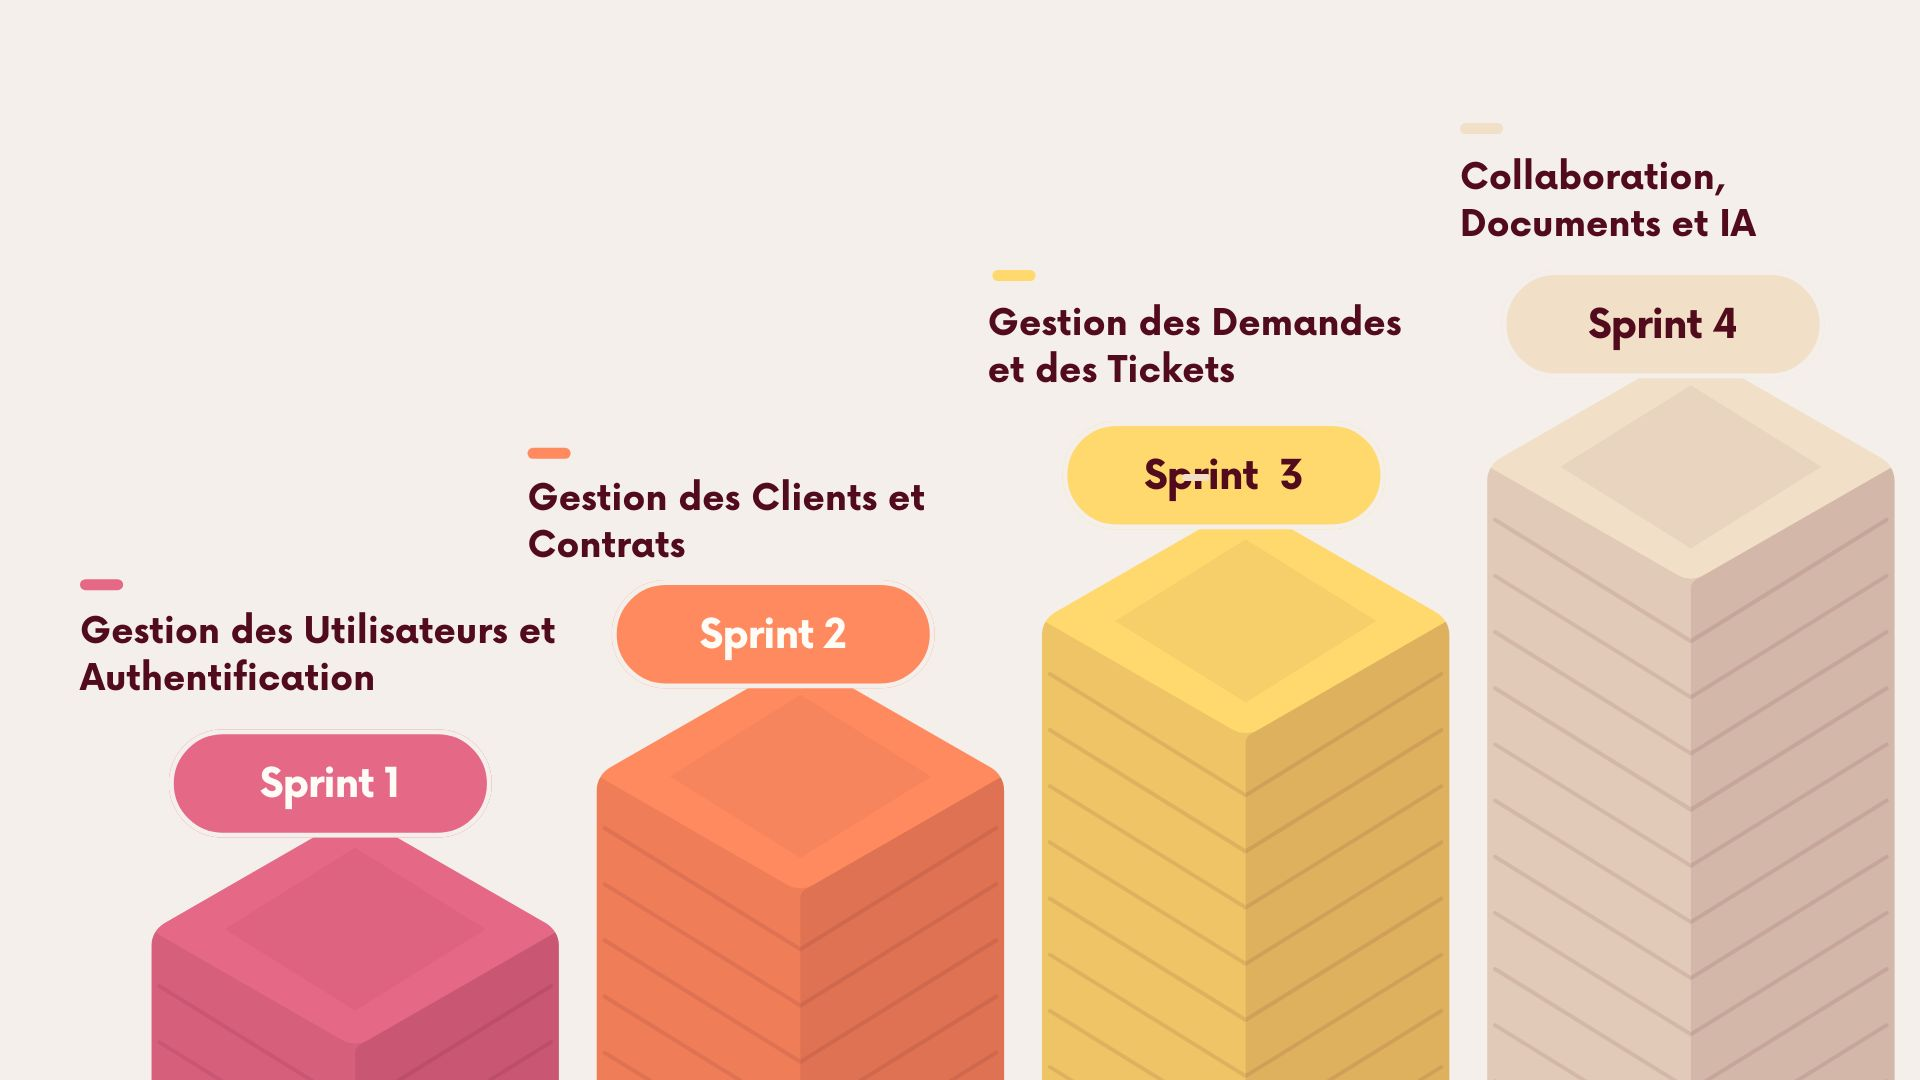
\includegraphics[width=0.8\textwidth,keepaspectratio]{Images/Scrum planning.jpg}
\caption{Planification chronologique des sprints}
\label{fig:planification_sprints}
\end{figure}

\subsubsection{Sprint 1 -- Authentification, Sécurité et Gestion des Utilisateurs}
\textbf{Période :} du 17 février au 11 mars (\textbf{3 semaines})
\newline
\textbf{Objectif du sprint :} Mettre en place le système d'authentification sécurisé
et la gestion complète des utilisateurs avec contrôle d'accès basé sur
les rôles (RBAC).

\noindent\textbf{User Stories sélectionnées :}
\begin{itemize}[nosep,leftmargin=1.6cm,topsep=0pt,itemsep=2pt,label=$\bullet$]
  \item \textbf{Epic 1 -- Authentification et Sécurité} : US01 à US05 (5 user stories)
  \item \textbf{Epic 2 -- Gestion des utilisateurs} : US06 à US11 (6 user stories)
  \item \textbf{Epic 3 -- Gestion des rôles et permissions} : US12 à US14 (3 user stories)
  \item \textbf{Epic 4 -- Demandes d'inscription OAuth} : US15 à US16 (2 user stories)
\end{itemize}

\noindent\textbf{Livrables attendus :}
\begin{itemize}[nosep,leftmargin=1.6cm,topsep=0pt,itemsep=2pt,label=$\bullet$]
  \item Système d'authentification fonctionnel (JWT + OAuth Google/GitHub)
  \item Module de gestion des utilisateurs avec verrouillage de compte
  \item Système RBAC complet avec gestion des rôles et permissions granulaires
\end{itemize}

\subsubsection{Sprint 2 -- Gestion des Clients, Projets et Contrats}
\textbf{Période :} du 12 mars au 2 avril (\textbf{3 semaines})
\newline
\textbf{Objectif du sprint :} Développer la gestion complète des clients, des projets et contrats
de maintenance avec système d'alertes d'expiration et configuration SLA.

\noindent
\textbf{User Stories sélectionnées :}
\begin{itemize}[nosep,leftmargin=1.6cm,topsep=0pt,itemsep=2pt,label=$\bullet$]
  \item \textbf{Epic 5 -- Gestion des clients et projets} : US17 à US26 (10 user stories)
  \item \textbf{Epic 6 -- Gestion des contrats} : US27 à US37 (10 user stories)
  \item \textbf{Epic 14 -- Historique et traçabilité} : US101 à US102 (2 user stories)
\end{itemize}

\noindent\textbf{Livrables attendus :}
\begin{itemize}[nosep,leftmargin=1.6cm,topsep=0pt,itemsep=2pt,label=$\bullet$]
  \item Module de gestion des clients avec profils société
  \item Module de gestion des projets avec équipes et membres
  \item Système de gestion des contrats avec SLA, alertes à J-30/J-15/J-7 et
    workflow d'approbation
  \item Système d'audit et traçabilité complet (ActivityLog)
\end{itemize}

\subsubsection{Sprint 3 -- Gestion des Demandes et Tickets}
\textbf{Période :} du 3 avril au 24 avril (\textbf{4 semaines})
\newline
\textbf{Objectif du sprint :} Implémenter le cœur métier avec la gestion des
demandes et tickets incluant suivi du temps, SLA et tableau Kanban.

\noindent\textbf{User Stories sélectionnées :}
\begin{itemize}[nosep,leftmargin=1.6cm,topsep=0pt,itemsep=2pt,label=$\bullet$]
  \item \textbf{Epic 7 -- Gestion des demandes} : US38 à US44 (7 user stories)
  \item \textbf{Epic 8 -- Gestion des tickets} : US45 à US64 (20 user stories)
  \item \textbf{Epic 15 -- Intelligence Artificielle} : US105 à US110 (6 user stories)
\end{itemize}

\noindent\textbf{Livrables attendus :}
\begin{itemize}[nosep,leftmargin=1.6cm,topsep=0pt,itemsep=2pt,label=$\bullet$]
  \item Module de gestion des demandes de maintenance avec classification
  \item Système complet de gestion des tickets avec vue Kanban (drag \& drop)
  \item Chronomètre de travail par session et respect des SLA en minutes ouvrées
  \item Moteur d'IA pour classification automatique des demandes et assistance intelligente
\end{itemize}

\subsubsection{Sprint 4 -- Collaboration, Documents et Planification}
\textbf{Période :} du 25 avril au 22 mai (\textbf{3 semaines})
\par\noindent\textbf{Objectif du sprint :} Finaliser les fonctionnalités avancées de
collaboration, de gestion documentaire, de notifications multicanales et de
planification.

\noindent\textbf{User Stories sélectionnées :}
\begin{itemize}[nosep,leftmargin=1.6cm,topsep=0pt,itemsep=2pt,label=$\bullet$]
  \item \textbf{Epic 9 -- Calendrier et planification} : US65 à US68 (4 user stories)
  \item \textbf{Epic 10 -- Messagerie et collaboration} : US69 à US77 (9 user stories)
  \item \textbf{Epic 11 -- Gestion des documents} : US78 à US88 (11 user stories)
  \item \textbf{Epic 12 -- Notifications et alertes} : US89 à US93 (5 user stories)
  \item \textbf{Epic 13 -- Dashboards et rapports} : US94 à US100 (7 user stories)
  \item \textbf{Epic 14 -- Historique et traçabilité} : US103 à US104 (2 user stories)
\end{itemize}

\noindent
\textbf{Livrables attendus :}
\begin{itemize}[nosep,leftmargin=1.6cm,topsep=0pt,itemsep=2pt,label=$\bullet$]
  \item Système de messagerie et collaboration temps réel (WebSocket)
  \item Module de gestion documentaire avec versioning et base de connaissances
  \item Système de notifications multicanaux (in-app, email, Slack et Web Push)
  \item Module de génération de rapports et procès-verbaux PDF
  \item Tableaux de bord pour pilotage et calendrier de planification
  \item Système de traçabilité et historique des activités
\end{itemize}

\noindent\textbf{Synthèse de la planification :} Cette répartition assure une
progression logique où chaque sprint s'appuie sur les livrables précédents. Les
dépendances techniques sont respectées (authentification avant tickets, contrats
avant demandes), et la valeur métier croît progressivement jusqu'aux fonctionnalités
différenciantes du sprint final.

\subsection{Planning prévisionnel (Diagramme de Gantt)}
\label{sec:planning}
« Un diagramme de Gantt est un outil d'organisation et de gestion de projets. Il
s'agit d'un diagramme à barres horizontales qui présente toutes les tâches d'un
projet en fonction d'un calendrier. Il aide les chefs de projet à visualiser les
tâches requises et à suivre l'avancement de leur projet. » [5]
\newline
Dans le cadre du développement de notre projet \textbf{SolidMaint}, le planning
prévisionnel a été réalisé pour organiser les différentes phases de développement.
La figure ci-dessous illustre cette planification :

\begin{figure}[H]
\centering
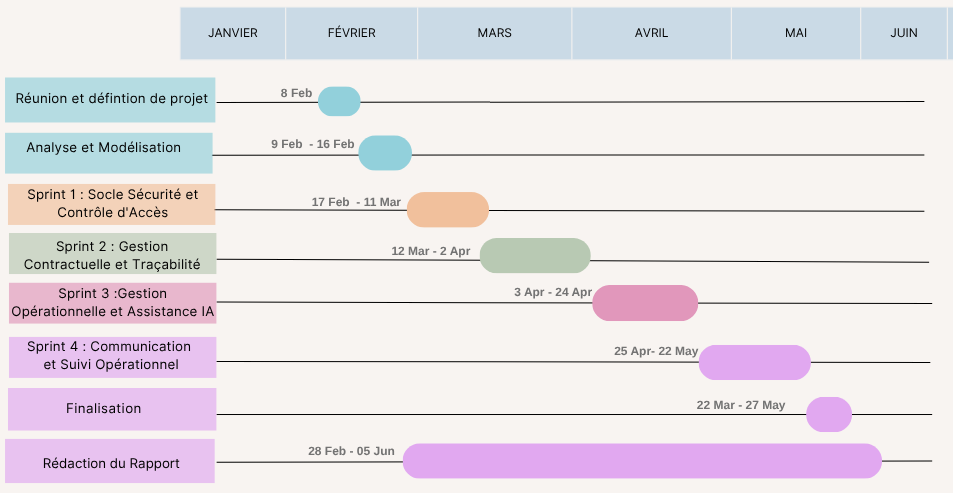
\includegraphics[width=0.7\textwidth,keepaspectratio]{Images/Diagramme_Gantt.png}
\caption{Diagramme de Gantt}
\end{figure}

%─────────────────────────────────────────────────────────────────────────────
% SECTION IV : ENVIRONNEMENT DE DÉVELOPPEMENT
%─────────────────────────────────────────────────────────────────────────────

\section{Environnement de Développement}
\label{sec:environnement}
On va commencer par la présentation de l'environnement matériel et logiciel que nous
utilisons.

\subsection{Environnement matériel}
\begin{table}[H]
\centering
\renewcommand{\arraystretch}{1.6}
\arrayrulecolor{gray!70}
\rowcolors{2}{gray!5}{white}
\begin{tabularx}{\textwidth}{| >{\centering\arraybackslash}X
                              | >{\centering\arraybackslash}X
                              | >{\centering\arraybackslash}X |}
\rowcolor{blue!20} \hline
\textbf{Ordinateur}        & \textbf{1}                          & \textbf{2}          \\
\hline
Propriétaire               & Rihab Chourou                       & Eya Gharbi          \\
\hline
Processeur                 & Core i3                             & Core i3             \\
\hline
RAM                        & 20 Go                               & 16 Go               \\
\hline
Disque dur                 & 1 To                                & 256 Go              \\
\hline
Système d'exploitation     & Windows 10 Professionnel N 64-bit   & Windows 10 Professionnel 64-bit \\
\hline
\end{tabularx}
\caption{Environnement matériel de développement}
\label{tab:environnement_de_developpement}
\end{table}

\subsection{Environnement logiciel}

\subsubsection{Langages de programmation et frameworks}
\vspace{12pt}

\newcommand{\cadretech}[2]{%
\noindent\begin{minipage}{1.8cm}\centering
  \includegraphics[width=1.5cm,keepaspectratio]{#1}
\end{minipage}\hspace{0.5cm}%
\begin{minipage}{\dimexpr\textwidth-1.8cm-0.5cm-2\fboxsep-2\fboxrule\relax}
  \fbox{\parbox{\dimexpr\linewidth-2\fboxsep\relax}{#2}}
\end{minipage}\par\vspace{10pt}}

\cadretech{Images/nestjs.png}{%
  \textbf{NestJS v11 :} « C'est un framework permettant de créer des applications
  serveur Node.js performantes et évolutives. Il utilise JavaScript progressif, est
  conçu avec TypeScript et le prend entièrement en charge (tout en permettant aux
  développeurs de coder en JavaScript pur). » [6]}

\cadretech{Images/nextjs.png}{%
  \textbf{Next.js v16 :} « C'est un framework React permettant de créer des
  applications web complètes. Il configure également automatiquement les outils de
  bas niveau tels que les modules de regroupement et les compilateurs. » [7]}

\cadretech{Images/React-icon.png}{%
  \textbf{React 18.3 :} « React est une bibliothèque JavaScript pour la construction
  d'interfaces utilisateur. Elle permet de créer des composants réutilisables qui
  gèrent leur propre état et se composent pour former des interfaces complexes. » [8]}

\cadretech{Images/Tailwind.png}{%
  \textbf{Tailwind CSS v4.2 :} « Un framework CSS utilitaire, doté de classes telles
  que \texttt{flex}, \texttt{pt-4}, \texttt{text-center} et \texttt{rotate-90}, qui
  peuvent être combinées pour créer n'importe quel design, directement dans votre
  balisage. » [9]}

\cadretech{Images/chadcn.png}{%
  \textbf{shadcn/ui v3.8 :} « est un ensemble de composants élégants et accessibles,
  ainsi qu'une plateforme de distribution de code. Compatible avec vos frameworks et
  modèles d'IA préférés. Logiciel libre. » [10]}

\subsubsection{Outils de développement et modélisation}
\vspace{12pt}

\newcommand{\cadretechVscode}[2]{%
\noindent\begin{minipage}{2.2cm}\centering
  \includegraphics[width=2cm,height=1.5cm,keepaspectratio]{#1}
\end{minipage}\hspace{0.5cm}%
\begin{minipage}{\dimexpr\textwidth-2.2cm-0.5cm-2\fboxsep-2\fboxrule\relax}
  \fbox{\parbox{\dimexpr\linewidth-2\fboxsep\relax}{#2}}
\end{minipage}\par\vspace{10pt}}

\cadretechVscode{Images/Visual_Studio_Code.png}{%
  \textbf{Visual Studio Code :} « est un éditeur de code source léger mais puissant,
  disponible sur Windows, macOS et Linux. Il intègre la coloration syntaxique, la
  complétion intelligente du code (IntelliSense), le débogage, le contrôle de version
  Git et une riche bibliothèque d'extensions. » [11]}

\newcommand{\cadretechGitlab}[2]{%
    \noindent
    \begin{minipage}{2.2cm}
        \centering
        \includegraphics[width=2cm, height=1.5cm, keepaspectratio]{#1}
    \end{minipage}
    \hspace{0.5cm}
    \begin{minipage}{\dimexpr\textwidth-2.2cm-0.5cm-2\fboxsep-2\fboxrule\relax}
        \fbox{%
            \parbox{\dimexpr\linewidth-2\fboxsep\relax}{%
                #2%
            }%
        }%
    \end{minipage}
    \par
    \vspace{10pt}
}
\cadretechGitlab{Images/gitlab.png}{ \textbf{GitLab : } « offre un espace de stockage de code en ligne ainsi que des fonctionnalités de suivi des problèmes et d'intégration continue/déploiement continu ( CI/CD). Le dépôt permet d'héberger différentes branches de développement et
  versions. » [12]}

\newcommand{\cadretechUml}[2]{%
\noindent\begin{minipage}{2.2cm}\centering
  \includegraphics[width=2cm,height=1.5cm,keepaspectratio]{#1}
\end{minipage}\hspace{0.5cm}%
\begin{minipage}{\dimexpr\textwidth-2.2cm-0.5cm-2\fboxsep-2\fboxrule\relax}
  \fbox{\parbox{\dimexpr\linewidth-2\fboxsep\relax}{#2}}
\end{minipage}\par\vspace{10pt}}

\cadretechUml{Images/uml.png}{%
  \textbf{UML :} « est un langage permettant de spécifier, visualiser, construire et
  documenter les artefacts des systèmes logiciels, ainsi que de modéliser des systèmes
  métier et d'autres systèmes non logiciels. L'UML représente un ensemble de bonnes
  pratiques d'ingénierie qui ont fait leurs preuves dans la modélisation de systèmes
  vastes et complexes. » [13]}

\newcommand{\cadretechDrowio}[2]{%
\noindent\begin{minipage}{2.2cm}\centering
  \includegraphics[width=2cm,height=1.5cm,keepaspectratio]{#1}
\end{minipage}\hspace{0.5cm}%
\begin{minipage}{\dimexpr\textwidth-2.2cm-0.5cm-2\fboxsep-2\fboxrule\relax}
  \fbox{\parbox{\dimexpr\linewidth-2\fboxsep\relax}{#2}}
\end{minipage}\par\vspace{10pt}}

\cadretechDrowio{Images/lucidchart.png}{%
  \textbf{Lucidchart :} « est un environnement de travail visuel qui associe création
  de diagrammes, visualisation de données et fonctionnalités de collaboration afin de
  faciliter la communication et stimuler l'innovation. » [14]}

\newcommand{\cadretechSwagger}[2]{%
\noindent\begin{minipage}{2.2cm}\centering
  \includegraphics[width=2cm,height=1.5cm,keepaspectratio]{#1}
\end{minipage}\hspace{0.5cm}%
\begin{minipage}{\dimexpr\textwidth-2.2cm-0.5cm-2\fboxsep-2\fboxrule\relax}
  \fbox{\parbox{\dimexpr\linewidth-2\fboxsep\relax}{#2}}
\end{minipage}\par\vspace{10pt}}

\cadretechSwagger{Images/swagger.png}{%
  \textbf{Swagger / OpenAPI :} « Swagger permet la conception, la gouvernance et les
  tests tout au long du cycle de vie complet des API, garantissant ainsi la qualité à
  chaque étape. Il génère automatiquement une documentation interactive de l'API à
  partir des annotations du code source. » [15]}

\subsubsection{Systèmes de gestion de bases de données}
\vspace{12pt}

\newcommand{\cadretechPrisma}[2]{%
\noindent\begin{minipage}{2.2cm}\centering
  \includegraphics[width=2cm,height=1.5cm,keepaspectratio]{#1}
\end{minipage}\hspace{0.5cm}%
\begin{minipage}{\dimexpr\textwidth-2.2cm-0.5cm-2\fboxsep-2\fboxrule\relax}
  \fbox{\parbox{\dimexpr\linewidth-2\fboxsep\relax}{#2}}
\end{minipage}\par\vspace{10pt}}

\cadretechPrisma{Images/prisma.png}{%
  \textbf{Prisma ORM v7 :} « est un ORM open source de nouvelle génération qui offre
  un accès rapide et sécurisé aux bases de données PostgreSQL, MySQL et autres. Il
  fournit un client typé généré automatiquement à partir du schéma de données,
  garantissant la sécurité des types à la compilation et des requêtes SQL optimisées
  à l'exécution. » [16]}

\newcommand{\cadretechPostgres}[2]{%
\noindent\begin{minipage}{2.2cm}\centering
  \includegraphics[width=2cm,height=1.5cm,keepaspectratio]{#1}
\end{minipage}\hspace{0.5cm}%
\begin{minipage}{\dimexpr\textwidth-2.2cm-0.5cm-2\fboxsep-2\fboxrule\relax}
  \fbox{\parbox{\dimexpr\linewidth-2\fboxsep\relax}{#2}}
\end{minipage}\par\vspace{10pt}}

\cadretechPostgres{Images/postgres.png}{%
  \textbf{PostgreSQL 16 :} « est un système de gestion de bases de données
  objet-relationnelles (SGBD-OR) open source. Il a été pionnier dans de nombreux
  concepts qui ne sont devenus disponibles que bien plus tard dans certains systèmes
  de bases de données commerciaux. Il est reconnu pour sa robustesse, sa conformité
  aux standards SQL et ses performances sur de grands volumes de données. » [17]}

\newcommand{\cadretechRedis}[2]{%
\noindent\begin{minipage}{2.2cm}\centering
  \includegraphics[width=2cm,height=1.5cm,keepaspectratio]{#1}
\end{minipage}\hspace{0.5cm}%
\begin{minipage}{\dimexpr\textwidth-2.2cm-0.5cm-2\fboxsep-2\fboxrule\relax}
  \fbox{\parbox{\dimexpr\linewidth-2\fboxsep\relax}{#2}}
\end{minipage}\par\vspace{10pt}}

\cadretechRedis{Images/redis.jpg}{%
  \textbf{Redis 7 :} « est un système de stockage de données en mémoire open source,
  utilisé comme base de données, cache et courtier de messages. Sa structure de
  données en mémoire vive lui confère des performances de lecture/écriture
  exceptionnellement rapides. Dans notre projet, Redis est utilisé comme couche de
  cache pour les permissions utilisateurs et les données fréquemment consultées,
  avec une durée de vie (TTL) de 60 secondes. » [18]}

\newcommand{\cadretechNeon}[2]{%
\noindent\begin{minipage}{2.2cm}\centering
  \includegraphics[width=2cm,height=1.5cm,keepaspectratio]{#1}
\end{minipage}\hspace{0.5cm}%
\begin{minipage}{\dimexpr\textwidth-2.2cm-0.5cm-2\fboxsep-2\fboxrule\relax}
  \fbox{\parbox{\dimexpr\linewidth-2\fboxsep\relax}{#2}}
\end{minipage}\par\vspace{10pt}}

\cadretechNeon{Images/Neon.png}{%
  \textbf{Neon :} « est un service de base de données PostgreSQL cloud natif, sans
  serveur et entièrement managé. Il offre une mise à l'échelle automatique, une
  séparation calcul/stockage et une compatibilité totale avec PostgreSQL, permettant
  de démarrer sans infrastructure à gérer. » [19]}

\subsubsection{Conteneurisation et déploiement}
\vspace{12pt}

\newcommand{\cadretechDocker}[2]{%
\noindent\begin{minipage}{2.2cm}\centering
  \includegraphics[width=2cm,height=1.5cm,keepaspectratio]{#1}
\end{minipage}\hspace{0.5cm}%
\begin{minipage}{\dimexpr\textwidth-2.2cm-0.5cm-2\fboxsep-2\fboxrule\relax}
  \fbox{\parbox{\dimexpr\linewidth-2\fboxsep\relax}{#2}}
\end{minipage}\par\vspace{10pt}}

\cadretechDocker{Images/docker.png}{%
  \textbf{Docker et Docker Compose :} « Docker est une plateforme open source qui
  permet d'automatiser le déploiement d'applications dans des conteneurs logiciels
  légers et portables. Docker Compose permet de définir et d'exécuter des
  applications multi-conteneurs à l'aide d'un fichier de configuration YAML. Dans
  notre projet, Docker Compose orchestre quatre services : PostgreSQL, Redis, le
  backend NestJS et le frontend Next.js. » [20]}
  
\subsubsection{Référentiel de sécurité applicative}
\vspace{12pt}
\newcommand{\cadretechSecurite}[2]{%
\noindent\begin{minipage}{2.2cm}\centering
  \includegraphics[width=2cm,height=1.5cm,keepaspectratio]{#1}
\end{minipage}\hspace{0.5cm}%
\begin{minipage}{\dimexpr\textwidth-2.2cm-0.5cm-2\fboxsep-2\fboxrule\relax}
  \fbox{\parbox{\dimexpr\linewidth-2\fboxsep\relax}{#2}}
\end{minipage}\par\vspace{10pt}}

\cadretechSecurite{Images/owasp.png}{%
  \textbf{OWASP ZAP :} « L'Open Worldwide Application Security Project (OWASP) est une fondation à but non lucratif qui œuvre pour améliorer la sécurité des logiciels. Dans le cadre de ce projet, l'outil OWASP ZAP a été utilisé pour réaliser des scans automatisés de vulnérabilités sur l'ensemble des endpoints exposés par l'application. » [21]}

\subsubsection{Outils de test}
\vspace{12pt}

\newcommand{\cadretechksix}[2]{%
\noindent\begin{minipage}{2.2cm}\centering
  \includegraphics[width=2cm,height=1.5cm,keepaspectratio]{#1}
\end{minipage}\hspace{0.5cm}%
\begin{minipage}{\dimexpr\textwidth-2.2cm-0.5cm-2\fboxsep-2\fboxrule\relax}
  \fbox{\parbox{\dimexpr\linewidth-2\fboxsep\relax}{#2}}
\end{minipage}\par\vspace{10pt}}

\cadretechksix{Images/k6.png}{%
  \textbf{Grafana k6 :} « est un outil de test de performance open source, convivial pour les développeurs et extensible, qui vous aide à détecter rapidement les problèmes de performance et à améliorer proactivement la fiabilité. » [22]}

\newcommand{\cadretechVitest}[2]{%
\noindent\begin{minipage}{2.2cm}\centering
  \includegraphics[width=2cm,height=1.5cm,keepaspectratio]{#1}
\end{minipage}\hspace{0.5cm}%
\begin{minipage}{\dimexpr\textwidth-2.2cm-0.5cm-2\fboxsep-2\fboxrule\relax}
  \fbox{\parbox{\dimexpr\linewidth-2\fboxsep\relax}{#2}}
\end{minipage}\par\vspace{10pt}}

\cadretechVitest{Images/vitest.png}{%
  \textbf{Vitest :} « est un framework de tests unitaires ultrarapide propulsé par Vite, conçu pour les projets JavaScript et TypeScript modernes. Il permet d'isoler et de valider le comportement de chaque service de manière indépendante grâce à un système de mocks performant. » [26]}

\newcommand{\cadretechPlaywright}[2]{%
\noindent\begin{minipage}{2.2cm}\centering
  \includegraphics[width=2cm,height=1.5cm,keepaspectratio]{#1}
\end{minipage}\hspace{0.5cm}%
\begin{minipage}{\dimexpr\textwidth-2.2cm-0.5cm-2\fboxsep-2\fboxrule\relax}
  \fbox{\parbox{\dimexpr\linewidth-2\fboxsep\relax}{#2}}
\end{minipage}\par\vspace{10pt}}

\cadretechPlaywright{Images/playwright.png}{%
  \textbf{Playwright :} « est un framework de tests End-to-End développé par Microsoft, permettant d'automatiser les interactions avec un navigateur réel. Il a été utilisé pour valider les parcours utilisateur complets en simulant les actions réelles sur l'interface graphique de la plateforme. » [27]}

\subsubsection{Outil de gestion de projet Scrum}
\vspace{12pt}

\newcommand{\cadretechNotion}[2]{%
\noindent\begin{minipage}{2.2cm}\centering
  \includegraphics[width=2cm,height=1.5cm,keepaspectratio]{#1}
\end{minipage}\hspace{0.5cm}%
\begin{minipage}{\dimexpr\textwidth-2.2cm-0.5cm-2\fboxsep-2\fboxrule\relax}
  \fbox{\parbox{\dimexpr\linewidth-2\fboxsep\relax}{#2}}
\end{minipage}\par\vspace{10pt}}

\cadretechNotion{Images/Notion.png}{%
  \textbf{Notion :} « est un puissant outil no-code de productivité. Il aide à gérer
  une base de connaissances, pour rendre plus facile et convivial le travail au sein
  des collaborateurs. Cette application se révèle indispensable autant pour les
  travailleurs autonomes que pour les professionnels en entreprise. C'est également
  un outil parfait pour gérer son projet agile (Product Backlog, suivi des sprints,
  rétrospectives). » [23]}

\subsubsection{Environnement de composition de documents}
\vspace{12pt}

\newcommand{\cadretechLatex}[2]{%
\noindent\begin{minipage}{2.2cm}\centering
  \includegraphics[width=2cm,height=1.5cm,keepaspectratio]{#1}
\end{minipage}\hspace{0.5cm}%
\begin{minipage}{\dimexpr\textwidth-2.2cm-0.5cm-2\fboxsep-2\fboxrule\relax}
  \fbox{\parbox{\dimexpr\linewidth-2\fboxsep\relax}{#2}}
\end{minipage}\par\vspace{10pt}}

\cadretechLatex{Images/latex.png}{%
  \textbf{\LaTeX :} « est un système de composition de haute qualité ; il comprend
  des fonctionnalités conçues pour la production de documents techniques et
  scientifiques. \LaTeX{} est la norme de facto pour la communication et la
  publication de documents scientifiques. » [24]}

\subsubsection{Outil de design graphique}
\vspace{12pt}

\newcommand{\cadretechCanva}[2]{%
\noindent\begin{minipage}{2.2cm}\centering
  \includegraphics[width=2cm,height=1.5cm,keepaspectratio]{#1}
\end{minipage}\hspace{0.5cm}%
\begin{minipage}{\dimexpr\textwidth-2.2cm-0.5cm-2\fboxsep-2\fboxrule\relax}
  \fbox{\parbox{\dimexpr\linewidth-2\fboxsep\relax}{#2}}
\end{minipage}\par\vspace{10pt}}

\cadretechCanva{Images/canva.png}{%
  \textbf{Canva :} « est une plateforme de conception et de communication visuelle
  en ligne dont la mission est de permettre à chacun dans le monde de concevoir
  n'importe quoi et de publier n'importe où. » [25]}

\subsubsection{Logo de SolidMaint}
\vspace{0.4cm}
Le logo de \textbf{SolidMaint} a été conçu via \textbf{Canva} en cohérence avec la
charte visuelle de \textbf{SolidWall Consulting}. Il associe le \textbf{noir} et le
\textbf{jaune doré} à des symboles évocateurs de maintenance, de sécurité et de
traçabilité.

\begin{figure}[H]
\centering

\includegraphics[width=0.10\textwidth]{Images/solidmaint.png}
\caption{Logo de SolidMaint}
\label{fig:logo_solidmaint}
\end{figure}

%─────────────────────────────────────────────────────────────────────────────
% SECTION V : ARCHITECTURE DE L'APPLICATION
%─────────────────────────────────────────────────────────────────────────────

\section{Architecture de l'application}

\subsection{Architecture physique}
L'architecture système est un ensemble de décisions de conception qui définit
l'interaction des composants entre eux. Le choix de l'architecture est très sensible
car elle permet d'optimiser les performances du système et facilite son évolution en
fonction des volumes de données.
La figure ci-dessous montre l'architecture physique de notre application :

\begin{figure}[H]
\centering
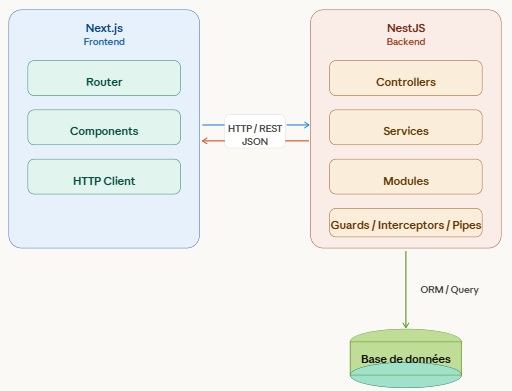
\includegraphics[width=0.7\textwidth,keepaspectratio]{Images/architecture.png}
\caption{Architecture physique de SolidMaint}
\label{fig:architecture_physique}
\end{figure}

\subsection{Architecture logique}
Nous avons choisi comme architecture logicielle l'\textbf{architecture monolithique
modulaire}. Ce choix est basé sur la combinaison entre la simplicité et la robustesse
des applications monolithiques traditionnelles, tout en bénéficiant de la clarté
structurelle des architectures orientées modules.

L'architecture du \textbf{monolithe modulaire} nous permet de travailler dans une
base de code unifiée, avec des frontières clairement définies et des modules
indépendants. Elle consiste à diviser le système en plusieurs modules fonctionnels
cohésifs, chacun encapsulant sa propre logique métier, ses contrôleurs, ses services
et ses DTOs.

Nous avons choisi cette architecture afin de maintenir l'indépendance des modules et
d'obtenir une grande cohésion, une encapsulation des données, ainsi qu'une
focalisation sur les fonctionnalités métiers, tout en conservant la simplicité de
déploiement d'un monolithe.

\begin{figure}[H]
\centering
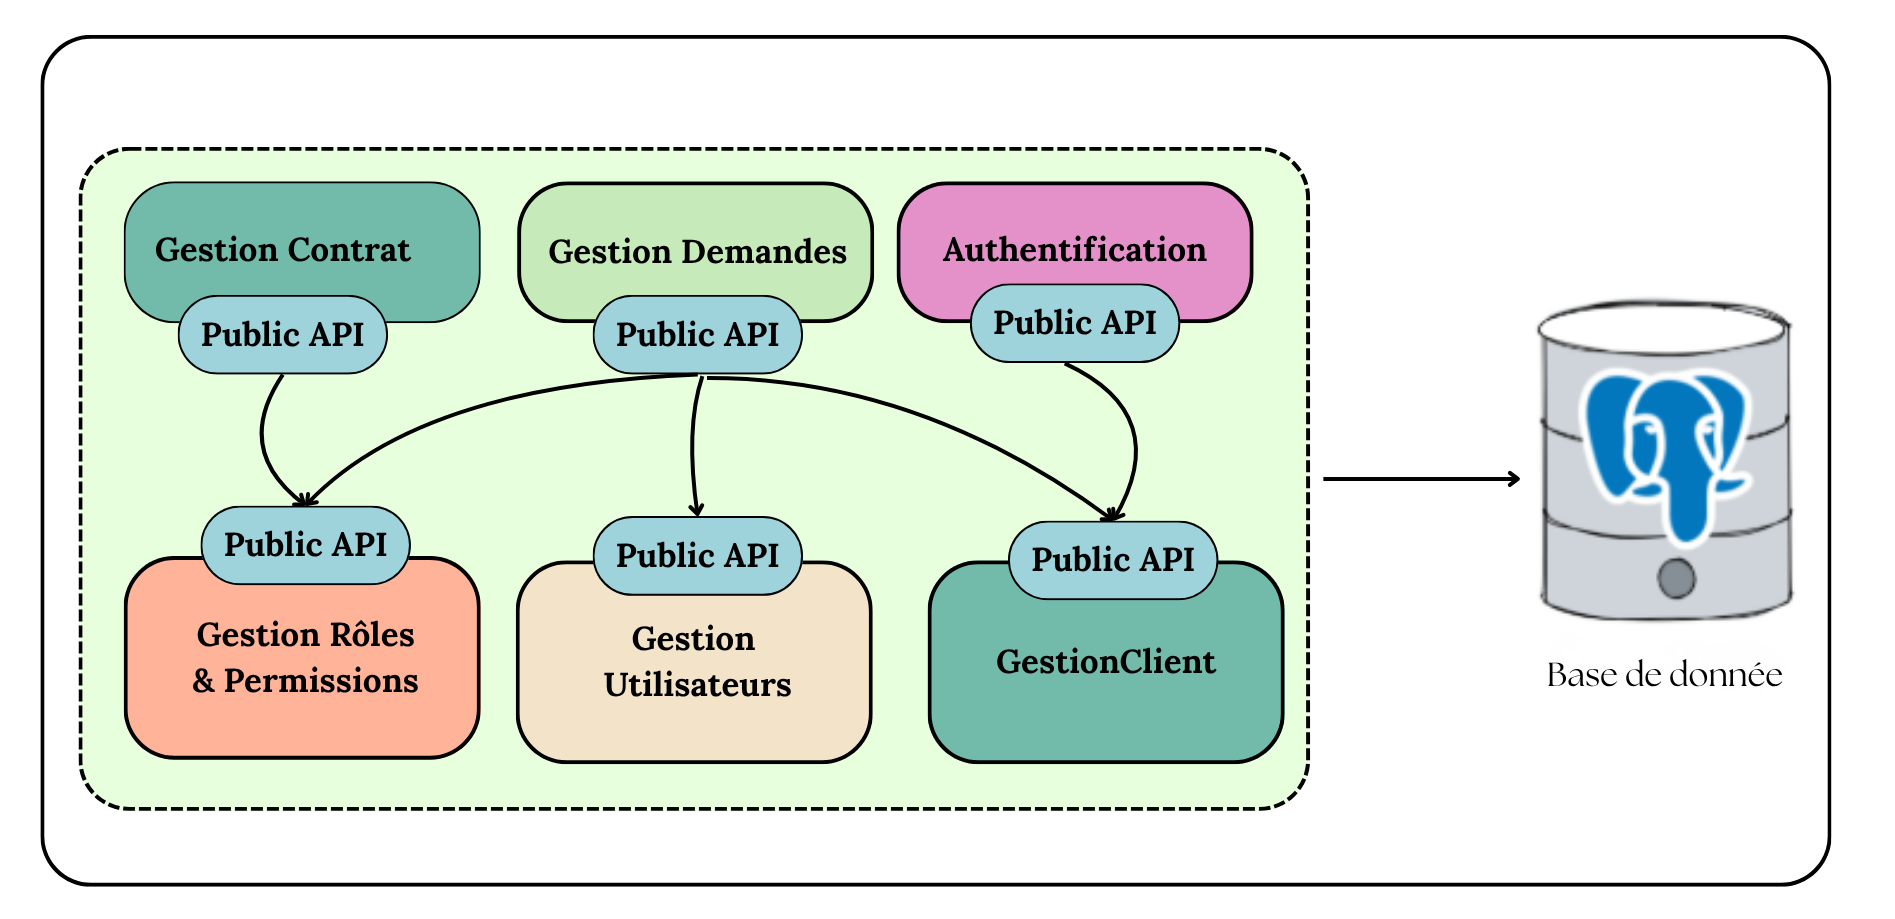
\includegraphics[width=0.7\textwidth,keepaspectratio]{Images/Modular Monoith.png}
\caption{Architecture monolithique modulaire}
\label{fig:architecture_modulaire}
\end{figure}

%─────────────────────────────────────────────────────────────────────────────
% CONCLUSION
%─────────────────────────────────────────────────────────────────────────────

\section{Conclusion}
Ce chapitre a établi les fondements techniques et méthodologiques de notre projet
\textbf{SolidMaint}. L'identification des six acteurs et la spécification des besoins
fonctionnels et non fonctionnels ont permis de définir précisément les exigences de
la plateforme. La modélisation UML et l'approche de pilotage Scrum avec la
planification en quatre sprints structurent la démarche de développement.

L'environnement de développement choisi et l'architecture modulaire garantissent une solution robuste et évolutive. Ces éléments constituent la base solide pour aborder la phase de réalisation.
\newline Le chapitre suivant détaillera l'implémentation du premier sprint consacré à la gestion des utilisateurs et authentification.

